%
% Main document
% ===========================================================================
% This is part of the document "Project documentation template".
% Authors: brd3, kaa1
%

%---------------------------------------------------------------------------
\documentclass[
	a4paper,					% paper format
	12pt,							% fontsize
%	twoside,					% double-sided
	openright,				% begin new chapter on right side
	notitlepage,			% use no standard title page
	parskip=half,			% set paragraph skip to half of a line
]{scrreprt}					% KOMA-script report
%---------------------------------------------------------------------------

\raggedbottom
\KOMAoptions{cleardoublepage=plain}			% Add header and footer on blank pages


% Load Standard Packages:
%---------------------------------------------------------------------------
\usepackage[standard-baselineskips]{cmbright}

\usepackage[ngerman]{babel}										% german hyphenation
\usepackage{afterpage}
%\usepackage[latin1]{inputenc}  							% Unix/Linux - load extended character set (ISO 8859-1)
\usepackage[ansinew]{inputenc}  							% Windows - load extended character set (ISO 8859-1)
\usepackage[T1]{fontenc}											% hyphenation of words with �,� and �
\usepackage{textcomp}													% additional symbols
\usepackage{longtable}
\usepackage{tabularx}
\usepackage{ae}																% better resolution of Type1-Fonts 
\usepackage{nameref}
\usepackage{floatrow}
\usepackage{wrapfig}
\usepackage{fancyhdr}													% simple manipulation of header and footer 
\usepackage{etoolbox}													% color manipulation of header and footer
\usepackage{graphicx}                      		% integration of images
\usepackage{float}														% floating objects
\usepackage{caption}													% for captions of figures and tables
\usepackage{subcaption}
\usepackage{booktabs}													% package for nicer tables
\usepackage{tocvsec2}													% provides means of controlling the sectional numbering
%\usepackage[style=verbose]{biblatex}
\usepackage{array}
\usepackage{algorithm}
\usepackage[noend]{algpseudocode}

%\usepackage{rotating}
\usepackage{pdflscape}
\usepackage{enumitem}
%\usepackage{svg}
%---------------------------------------------------------------------------

% Load Math Packages
%---------------------------------------------------------------------------
\usepackage{amsmath}                    	   	% various features to facilitate writing math formulas
\usepackage{amsthm}                       	 	% enhanced version of latex's newtheorem
\usepackage{amsfonts}                      		% set of miscellaneous TeX fonts that augment the standard CM
\usepackage{amssymb}													% mathematical special characters
\usepackage{exscale}													% mathematical size corresponds to textsize
%---------------------------------------------------------------------------

% Package to facilitate placement of boxes at absolute positions
%---------------------------------------------------------------------------
\usepackage[absolute]{textpos}
\setlength{\TPHorizModule}{1mm}
\setlength{\TPVertModule}{1mm}
%---------------------------------------------------------------------------					
			
% Definition of Colors
%---------------------------------------------------------------------------
\RequirePackage{color}                          % Color (not xcolor!)
\definecolor{linkblue}{rgb}{0,0,0.8}            % Standard
\definecolor{darkblue}{rgb}{0,0.08,0.45}        % Dark blue
\definecolor{bfhgrey}{rgb}{0.41,0.49,0.57}      % BFH grey
%\definecolor{linkcolor}{rgb}{0,0,0.8}     			% Blue for the web- and cd-version!
\definecolor{linkcolor}{rgb}{0,0,0}        			% Black for the print-version!
%---------------------------------------------------------------------------

% Hyperref Package (Create links in a pdf)
%---------------------------------------------------------------------------
\usepackage[
	pdftex,ngerman,bookmarks,plainpages=false,pdfpagelabels,
	backref = {false},										% No index backreference
	colorlinks = {true},                  % Color links in a PDF
	hypertexnames = {true},               % no failures "same page(i)"
	bookmarksopen = {true},               % opens the bar on the left side
	bookmarksopenlevel = {0},             % depth of opened bookmarks
	pdftitle = {Template f�r Bachelor Thesis},	   	% PDF-property
	pdfauthor = {brd3},        					  % PDF-property
	pdfsubject = {LaTeX Template},        % PDF-property
	linkcolor = {linkcolor},              % Color of Links
	citecolor = {linkcolor},              % Color of Cite-Links
	urlcolor = {linkcolor},               % Color of URLs
]{hyperref}
%---------------------------------------------------------------------------
% Set up page dimension
%---------------------------------------------------------------------------
\usepackage{geometry}
\geometry{
	a4paper,
	left=28mm,
	right=15mm,
	top=30mm,
	headheight=20mm,
	headsep=10mm,
	textheight=242mm,
	footskip=15mm
}
%---------------------------------------------------------------------------

% Makeindex Package
%---------------------------------------------------------------------------
\usepackage{makeidx}                         		% To produce index
\makeindex                                    	% Index-Initialisation
%---------------------------------------------------------------------------

% Glossary Package
%---------------------------------------------------------------------------
% the glossaries package uses makeindex
% if you use TeXnicCenter do the following steps:
%  - Goto "Ausgabeprofile definieren" (ctrl + F7)
%  - Select the profile "LaTeX => PDF"
%  - Add in register "Nachbearbeitung" a new "Postprozessoren" point named Glossar
%  - Select makeindex.exe in the field "Anwendung" ( ..\MiKTeX x.x\miktex\bin\makeindex.exe )
%  - Add this [ -s "%tm.ist" -t "%tm.glg" -o "%tm.gls" "%tm.glo" ] in the field "Argumente"
%
% for futher informations go to http://ewus.de/tipp-1029.html
%---------------------------------------------------------------------------
\usepackage[nonumberlist]{glossaries}
\makeglossaries
\usepackage{xparse}
\DeclareDocumentCommand{\newdualentry}{ O{} O{} m m m m } {
	\newglossaryentry{gls-#3}{name={#5},text={#5\glsadd{#3}},
		description={#6},#1
	}
	\newacronym[type=\acronymtype, see={[Glossary:]{gls-#3}},#2]{#3}{#4}{#5\glsadd{gls-#3}}
}


% GLOSSARY
\newglossaryentry{imvr}{name={IMVR},description={Kurz f�r ``Images \& Music in VR''. Die Applikation, die im Rahmen dieses Projekts mit Unity 5 entwickelt wird}}
\newglossaryentry{unity}{name={Unity},description={Unity ist eine Spielengine, die das einfache Entwickeln von 3D-Applikation f�r diverse Endger�te erlaubt}}
\newglossaryentry{rift}{name={Oculus Rift},description={Ein \gls{hmd} von Oculus VR}}
\newglossaryentry{leap}{name={Leap Motion},description={Ein auf Infrarotkameras basierter Handerkennungs-Sensor}}


% ACRONYMS
\newacronym[type=\acronymtype]{hmd}{HMD}{Head-Mounted Display}
\newacronym{vr}{VR}{Virtual Reality}
%\newglossaryentry{ipd}{name={IPD},description={Beschreibt den Augenabstand.}}
\newdualentry{ipd}{IPD}{Inter-Pupillary Distance}{Beschreibt den Augenabstand und stellt ein wichtiges Mass f�r die stereoskopische Darstellung von Bildern dar}
%\addbibresource{datenbanken/bibliography.bib}
%---------------------------------------------------------------------------

% Intro:
%---------------------------------------------------------------------------
\begin{document}                              	% Start Document
\settocdepth{section}														% Set depth of toc
\pagenumbering{roman}														
%---------------------------------------------------------------------------
\providecommand{\titel}{Bringing Your Hands Into Virtual Reality}		%  Hier den Titel des Berichts/Thesis eingeben					% Titel der Arbeit aus Datei titel.tex lesen
\providecommand{\versionnumber}{1.0}			%  Hier die aktuelle Versionsnummer eingeben
\providecommand{\versiondate}{11.06.2015}		%  Hier das Datum der aktuellen Version eingeben				% Versionsnummer und -datum aus Datei version.tex lesen

% Set up header and footer
%---------------------------------------------------------------------------
\makeatletter
\patchcmd{\@fancyhead}{\rlap}{\color{bfhgrey}\rlap}{}{}		% new color of header
\patchcmd{\@fancyfoot}{\rlap}{\color{bfhgrey}\rlap}{}{}		% new color of footer
\makeatother

\fancyhf{}																		% clean all fields
\fancypagestyle{plain}{												% new definition of plain style	
	\fancyfoot[OR,EL]{\footnotesize \thepage} 	% footer right part --> page number
	\fancyfoot[OL,ER]{\footnotesize \titel, Version \versionnumber, \versiondate}	% footer even page left part 
}

\renewcommand{\chaptermark}[1]{\markboth{\thechapter.  #1}{}}
\renewcommand{\headrulewidth}{0pt}				% no header stripline
\renewcommand{\footrulewidth}{0pt} 				% no bottom stripline

\newcommand{\code}{\texttt}

\newcommand\fnurl[2]{%
	\href{#2}{#1}\footnote{\url{#2}}%
}
\definecolor{light-gray}{gray}{0.95}
\lstset{language=[Sharp]C,
	showspaces=false,
	showtabs=false,
	breaklines=true,
	showstringspaces=false,
	breakatwhitespace=true,
	basewidth=0.5em,
	escapeinside={(*@}{@*)},
	commentstyle=\color{greencomments},
	keywordstyle=\color{bluekeywords},
	stringstyle=\color{redstrings},
	basicstyle=\ttfamily\small,
	captionpos=b,
%	backgroundcolor=\color{light-gray},
	xleftmargin=1cm,
	frame=tb,
	numbers={left}
}

\newcommand*{\captionsource}[2]{%
	\caption[{#1}]{%
		#1%
		\\\hspace{\linewidth}%
		\textbf{Source:} #2%
	}%
}

\newcommand{\source}[1]{\caption*{\hfill Quelle: {#1}} }

\pagestyle{plain}

%---------------------------------------------------------------------------


% Title Page and Abstract
%---------------------------------------------------------------------------
\newgeometry{twoside}
%%
% Project documentation template
% ===========================================================================
% This is part of the document "Project documentation template".
% Authors: brd3, kaa1
%

\begin{titlepage}


% BFH-Logo absolute placed at (28,12) on A4 
% Actually not a realy satisfactory solution but working.
%---------------------------------------------------------------------------
\setlength{\unitlength}{1mm}
\begin{textblock}{20}[0,0](28,12)
	
\includegraphics[scale=1.0]{bilder/BFH_Logo_B.png}
\end{textblock}
\color{black}

% Institution / Titel / Untertitel / Autoren / Experten:
%---------------------------------------------------------------------------
\begin{flushleft}

\vspace*{21mm}

\fontsize{26pt}{40pt}\selectfont 
\titel 				\\							% Titel aus der Datei vorspann/titel.tex lesen
\vspace{2mm}

\fontsize{16pt}{24pt}\selectfont\vspace{0.3em}
Hier steht ein Untertitel 			\\							% Untertitel eingeben
\vspace{5mm}

\fontsize{10pt}{12pt}\selectfont
\textbf{Art der Arbeit (Semesterarbeit / Bachelorthesis / etc.)} \\									% eingeben
\vspace{7mm}

% Abstract (eingeben):
%---------------------------------------------------------------------------
\begin{textblock}{150}(28,100)
\fontsize{10pt}{12pt}\selectfont
[Kurztext (Abstract) einf�gen, falls gew�nscht] \\ 
Dieses Dokument dient als Vorlage f�r die Erstellung von Berichten nach den Richtlinien der BFH. Die Vorlage ist in \LaTeX{} erstellt und unterst�tzt das automatische Erstellen von diversen Verzeichnissen, Literaturangaben, Indexierung und Glossaren. Dieser kleine Text ist eine Zusammenfassung �ber das vorliegenden Dokument mit einer L�nge von 4 bis max. 8 Zeilen. \\
Das Titelbild kann in den Zeilen 157/158 der Datei template.tex ein- oder ausgeschaltet werden.
\end{textblock}

\begin{textblock}{150}(28,225)
\fontsize{10pt}{17pt}\selectfont
\begin{tabbing}
xxxxxxxxxxxxxxx\=xxxxxxxxxxxxxxxxxxxxxxxxxxxxxxxxxxxxxxxxxxxxxxx \kill
Studiengang:	\> [z.B. Elektro- und Kommunikationstechnik]	\\			% Namen eingeben
Autoren:		\> [Test Peter, M�ster R�s�]		\\					% Namen eingeben
Betreuer:	\> [Dr.~Xxxx Xxxx, Dr.~Yyyy Yyyy]		\\					% Namen eingeben
Auftraggeber:	\> [Wwwww AG]						\\					% Namen eingeben
Experten:		\> [Dr.~Zzzz Zzzz]				\\					% Namen eingeben
Datum:			\> \versiondate					\\		% aus Datei vorspann/version.tex lesen
\end{tabbing}

\end{textblock}
\end{flushleft}

\begin{textblock}{150}(28,280)
\noindent 
\color{bfhgrey}\fontsize{9pt}{10pt}\selectfont
Berner Fachhochschule | Haute �cole sp�cialis�e bernoise | Bern University of Applied Sciences
\color{black}\selectfont
\end{textblock}


\end{titlepage}

%
% ===========================================================================
% EOF
%
		% activate for Titelseite ohne Bild
%
% Project documentation template
% ===========================================================================
% This is part of the document "Project documentation template".
% Authors: brd3, kaa1
%

\begin{titlepage}


% BFH-Logo absolute placed at (28,12) on A4 and picture (16:9 or 15cm x 8.5cm)
% Actually not a realy satisfactory solution but working.
%---------------------------------------------------------------------------
\setlength{\unitlength}{1mm}
\begin{textblock}{20}[0,0](28,12)
	
\includegraphics[scale=1.0]{bilder/BFH_Logo_B.png}
\end{textblock}

\begin{textblock}{154}(28,48)
	\begin{picture}(150,2)
		\put(0,0){\color{bfhgrey}\rule{150mm}{2mm}}
	\end{picture}
\end{textblock}

\begin{textblock}{154}[0,0](28,55)
	\centering
	
\includegraphics[width=0.7\linewidth]{bilder/logo}			% Titelbild definieren
\end{textblock}

\begin{textblock}{154}(28,155)
	\begin{picture}(150,2)
		\put(0,0){\color{bfhgrey}\rule{150mm}{2mm}}
	\end{picture}
\end{textblock}
\color{black}

% Institution / Titel / Untertitel / Autoren / Experten:
%---------------------------------------------------------------------------
\begin{flushleft}

\vspace*{125mm}

\fontsize{26pt}{28pt}\selectfont 
\titel 				\\							% Titel aus der Datei vorspann/titel.tex lesen
\vspace{2mm}

\fontsize{16pt}{20pt}\selectfont\vspace{0.3em}
Schlussbericht 			\\							% Untertitel eingeben
\vspace{5mm}

\fontsize{10pt}{12pt}\selectfont
%\textbf{Art der Arbeit (Semesterarbeit / Bachelorthesis / etc.)} \\									% eingeben
\vspace{3mm}

% Abstract (eingeben):
%---------------------------------------------------------------------------
%\begin{textblock}{150}(28,190)
%\fontsize{10pt}{12pt}\selectfont
%[Kurztext (Abstract) einf�gen, falls gew�nscht] \\ 
%Dieses Dokument dient als Vorlage f�r die Erstellung von Berichten nach den Richtlinien der BFH. Die Vorlage ist in \LaTeX{} erstellt und unterst�tzt das automatische Erstellen von diversen Verzeichnissen, Literaturangaben, Indexierung und Glossaren. Dieser kleine Text ist eine Zusammenfassung �ber das vorliegenden Dokument mit einer L�nge von 4 bis max. 8 Zeilen. \\
%Das Titelbild kann in den Zeilen 157/158 der Datei template.tex ein- oder ausgeschaltet werden.
%\end{textblock}

\begin{textblock}{150}(28,225)
\fontsize{10pt}{17pt}\selectfont
\begin{tabbing}
xxxxxxxxxxxxxxx\=xxxxxxxxxxxxxxxxxxxxxxxxxxxxxxxxxxxxxxxxxxxxxxx \kill
Studiengang:	\> Informatik	\\			% Namen eingeben
Autoren:		\> Simon Meer		\\					% Namen eingeben
Betreuer:	\> Prof. Urs K�nzler		\\					% Namen eingeben
%Auftraggeber:	\> [Wwwww AG]						\\					% Namen eingeben
Experten:		\> Yves Petitpierre				\\					% Namen eingeben
Datum:			\> \versiondate					\\		% aus Datei vorspann/version.tex lesen
\end{tabbing}

\end{textblock}
\end{flushleft}

\begin{textblock}{150}(28,280)
\noindent 
\color{bfhgrey}\fontsize{9pt}{10pt}\selectfont
Berner Fachhochschule | Haute �cole sp�cialis�e bernoise | Bern University of Applied Sciences
\color{black}\selectfont
\end{textblock}


\end{titlepage}

%
% ===========================================================================
% EOF
%
			% activate for Titelseite mit Bild
% Versionenkontrolle :
% -----------------------------------------------
%\pagebreak
\begin{textblock}{180}(15,150)
\color{black}
\begin{huge}
Versionen
\end{huge}
\vspace{10mm}

\fontsize{10pt}{18pt}\selectfont
\begin{tabbing}
xxxxxxxxxxx\=xxxxxxxxxxxxxxx\=xxxxxxxxxxxxxx\=xxxxxxxxxxxxxxxxxxxxxxxxxxxxxxxxxxxxxxxxxxxxxxx \kill
Version	\> Datum	\> Status		\> Bemerkungen		\\
0.9	\> 14.04.2015	\> Entwurf		\> Outline erstellt	\\
\end{tabbing}

\end{textblock}
%\pagebreak
\cleardoubleemptypage
\restoregeometry
\setcounter{page}{1}
%\cleardoublepage
%\phantomsection 
%\addcontentsline{toc}{chapter}{Management Summary}
%\chapter*{Management Summary}
\label{chap:managementSummary}

Lorem ipsum dolor sit amet, consectetur adipiscing elit. Phasellus scelerisque, leo sed iaculis ornare, mi leo semper urna, ac elementum libero est at risus. Donec eget aliquam urna. Lorem ipsum dolor sit amet, consectetur adipiscing elit. Nunc fermentum nunc sollicitudin leo porttitor volutpat. Duis ac enim lectus, quis malesuada lectus. Aenean vestibulum suscipit justo, in suscipit augue venenatis a. Donec interdum nibh ligula. Aliquam vitae dui a odio cursus interdum quis vitae mi. Phasellus ornare tortor fringilla velit accumsan quis tincidunt magna eleifend. Praesent nisl nibh, cursus in mattis ac, ultrices ac nulla. Nulla ante urna, aliquet eu tempus ut, feugiat id nisl. Nunc sit amet mauris vitae turpis scelerisque mattis et sed metus. Aliquam interdum congue odio, sed semper elit ullamcorper vitae. Morbi orci elit, feugiat vel hendrerit nec, sollicitudin non massa. Quisque lacus metus, vulputate id ullamcorper id, consequat eget orci \nocite{kopka:band1} \nocite{Marti06}. 

\cleardoubleemptypage
%---------------------------------------------------------------------------

% Table of contents
%---------------------------------------------------------------------------
\tableofcontents
\cleardoublepage
%---------------------------------------------------------------------------

% Main part:
%---------------------------------------------------------------------------
\pagenumbering{arabic}

\chapter{Einleitung}
\label{chap:einleitung}

Der Markt der stereoskopischen Brillen befindet sich in einem starken Wachstum. Oculus Rift, SteamVR, Project Morpheus, Nvidia VR - die Liste der teilnehmenden Partien w�chst und w�chst, doch neue Ausgabeger�te ben�tigen auch neue Eingabeger�te. Die Leap Motion kann als ein solches gez�hlt werden und bietet eine freie Handerkennung ohne irgendwelche Handschuhe tragen zu m�ssen.

In diesem Projekt geht es darum, die neuartige Eingabem�glichkeiten der Leap Motion in Verbindung mit der Oculus Rift einzusetzen und damit eine interaktive \gls{vr}-Applikation zu schreiben. Im Rahmen eines vorhergehenden Projekts wurde die Materie bereits bearbeitet und die M�glichkeiten erforscht. Es geht nun also haupts�chlich um die erfolgreiche Anwendung der erarbeiteten Informationen.
\chapter{Aufgabenstellung und Zielformulierung}

Jedes Projekt startet mit einer Aufgabenstellung. Im Falle dieses Projektes, hat sich diese im Laufe des Projekts ein wenig ge�ndert. Darauf soll ebenfalls eingegangen werden.

\section{Urspr�ngliche Zielformulierung}

Es soll eine Applikation namens ``\gls{imvr}'' entwickelt werden, welche Gebrauch von der Oculus Rift macht, um die Bilder- und Musiksammlung des Anwenders ansprechend darzustellen, z.B. in Form eines 3D-Karussels. Die zus�tzliche "Tiefe", die durch den Einsatz eines stereoskopischen \gls{hmd} entsteht, soll dem Anwender helfen, sich in seiner Medienbibliothek schneller zurechtzufinden.

Zus�tzlich dazu soll die Leap Motion dazu verwendet werden, um vollst�ndige Handfreiheit zu gew�hren: Der Anwender soll komplett ohne Maus und Tastatur imstande sein, sich durch seine Bilder zu navigieren.

Kurz zusammengefasst muss die Applikation:

\begin{itemize}
	\item Die Bild- und Musikbibliothek des Benutzers in stereoskopischem 3D darstellen.
	\item Diese freih�ndig durchsuchbar machen mit Sortier- und evtl. Gruppierfunktion.
	\item Die Bilder betrachtbar und die Musik abspielbar machen.
	\item Metainformationen darstellen (z.B. in Form von Diagrammen).
\end{itemize}

Zus�tzlich zur Applikation selbst soll noch ein zus�tzliches Tool entwickelt werden, welches im Voraus die Dateien auf dem Host-System indexiert und f�r die visuelle Applikation bereitstellt.

\section{�nderungen an der Zielformulierung}

Aufgrund der begrenzten Zeit und eines vermehrten Interesse in die Darstellung von Musik, wurde die Zielformulierung w�hrend des Projekts leicht abge�ndert. Neu wird die Bilderbibliothek des Anwenders komplett ignoriert, daf�r das Augenmerk auf seine Musikbibliothek gelegt.

Des Weiteren wurden auch �nderungen am Konzept der Applikation selbst vorgenommen. Dies ist auf die experimentelle Natur des Projekts zur�ckzuf�hren, da anfangs nicht klar ist, was funktioniert und was nicht. Konkret wurden zwei Modi eingef�hrt, und auf eine Sortier- und Gruppierfunktion verzichtet. Diese k�nnten allerdings in einem n�chsten Schritt eingebaut werden.

\section{Hilfsmittel \& Hardware}

Verschieden Hilfsmittel werden f�r die Durchf�hrung des Projektes gebraucht. Seitens Software sind diese:

\begin{table}[H]
	\caption{�bersicht der eingesetzten Software.}
	\centering
	\label{tab:software}
	\begin{tabular}{ l l l }
		\noalign{\smallskip} \hline \hline \noalign{\smallskip}
		\textbf{Name} & \textbf{Beschreibung} \\ \midrule
		Unity3D & Spielengine und Entwicklungsumgebung \\
		Visual Studio 2012 \& 2013 & Entwicklungsumgebung von Microsoft \\
		Blender & Open-Source 3D Modelling-Tool \\
		Krita & Open-Source Grafikbearbeitungs-Tool \\
		GIMP & Open-Source Grafikbearbeitungs-Tool \\
		LaTeX & Hilfsmittel f�r die Erstellung wissenschaftlicher Dokumente \\
		Microsoft Visio & Tool zur Erstellung von Diagrammen \\
		\noalign{\smallskip} \hline \noalign{\smallskip}
	\end{tabular}
\end{table}

Im Hardware-Departement wurde folgendes eingesetzt:

\begin{table}[H]
	\caption{�bersicht der eingesetzten Hardware.}
	\centering
	\label{tab:hardware}
	\begin{tabular}{ l l l }
		\noalign{\smallskip} \hline \hline \noalign{\smallskip}
		\textbf{Name} & \textbf{Beschreibung} \\ \midrule
		Oculus Rift & \gls{hmd} von Oculus VR \\
		Leap Motion & Hand- und Fingererkennungsger�t von Leap Motion, Inc. \\
		\noalign{\smallskip} \hline \noalign{\smallskip}
	\end{tabular}
\end{table}

F�r eine Erkl�rung der Oculus Rift und der Leap Motion sei an dieser Stelle auf das Pflichtenheft verwiesen.
\chapter{Design}

Bei der Entwicklung wurden diverse Design-Entscheidungen gef�llt, welche zum Teil bereits in einem Vorprojekt analysiert wurden. Diese sollen in diesem Kapitel aufgelistet und erl�utert werden. 

\section{System�bersicht}
\label{sec:sysoverview}
Um die Applikation zu bedienen, setzt der Anwender die Oculus Rift auf und bewegt sich im von der mitgelieferten Kamera erkennbaren Bereich.

Die Leap Motion wird prinzipiell so verwendet, wie von der Herstellerfirma vorgesehen. Das heisst, diese wird mit dem offiziellen Aufsatz \cite{leap} an der Oculus Rift befestigt, und deckt so den frontalen Sichtbereich des Anwenders ab. Dies l�sst sich gut auf Abbildung \ref{fig:systemuebersicht} erkennen.

Ebenfalls erkennbar ist, dass beide Ger�te per USB mit dem Host-Computer verbunden sind und Daten an die jeweiligen Services schicken. Diese Services werden durch die in Unity verwendeten Plugins angesteuert, und die ausgewerteten Daten in IMVR verwendet.

\afterpage {
	\begin{figure}[t!]
		\centering
		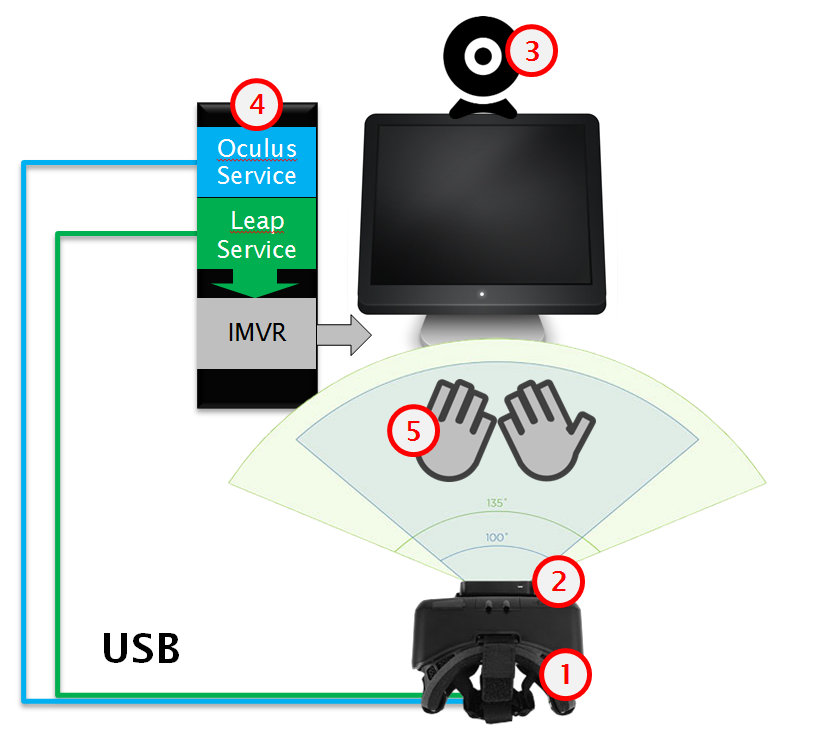
\includegraphics[width=0.8\linewidth]{bilder/systemuebersicht}
		\caption{Eine �bersicht der Technologien und wie sie verbunden sind.}
		\label{fig:systemuebersicht}
	\end{figure}
	
	\begin{table}[H]
		\centering
		\begin{tabular}{p{0.1\linewidth} p{0.3\linewidth} p{0.5\linewidth}}
			\textbf{Nr.} & \textbf{Komponente} & \textbf{Beschreibung} \\ \midrule
			1. & Oculus Rift DK2 & \gls{hmd} f�r den grafischen Output. \\
			2. & Leap Motion & Ger�t, welches H�nde erkennt und ihre Koordinaten an den Computer sendet. \\
			3. & Oculus Rift Kamera & Kamera, welche seit dem DK2 f�r das �rtliche Tracking zust�ndig ist. \\
			4. & Computer & Host-System f�r IMVR. \\
			5. & Benutzer & Benutzer, der die Oculus Rift tr�gt und mit seinen H�nden das Programm steuert. \\
		\end{tabular}
	\end{table}
}

\clearpage

\section{Systemarchitektur}

Zuerst ist es wichtig, zu verstehen, wie die Applikation grob aufgebaut ist. In Abbildung \ref{fig:flow} wird dies in zwei Schritten illustriert.

\begin{figure}[H]
\centering
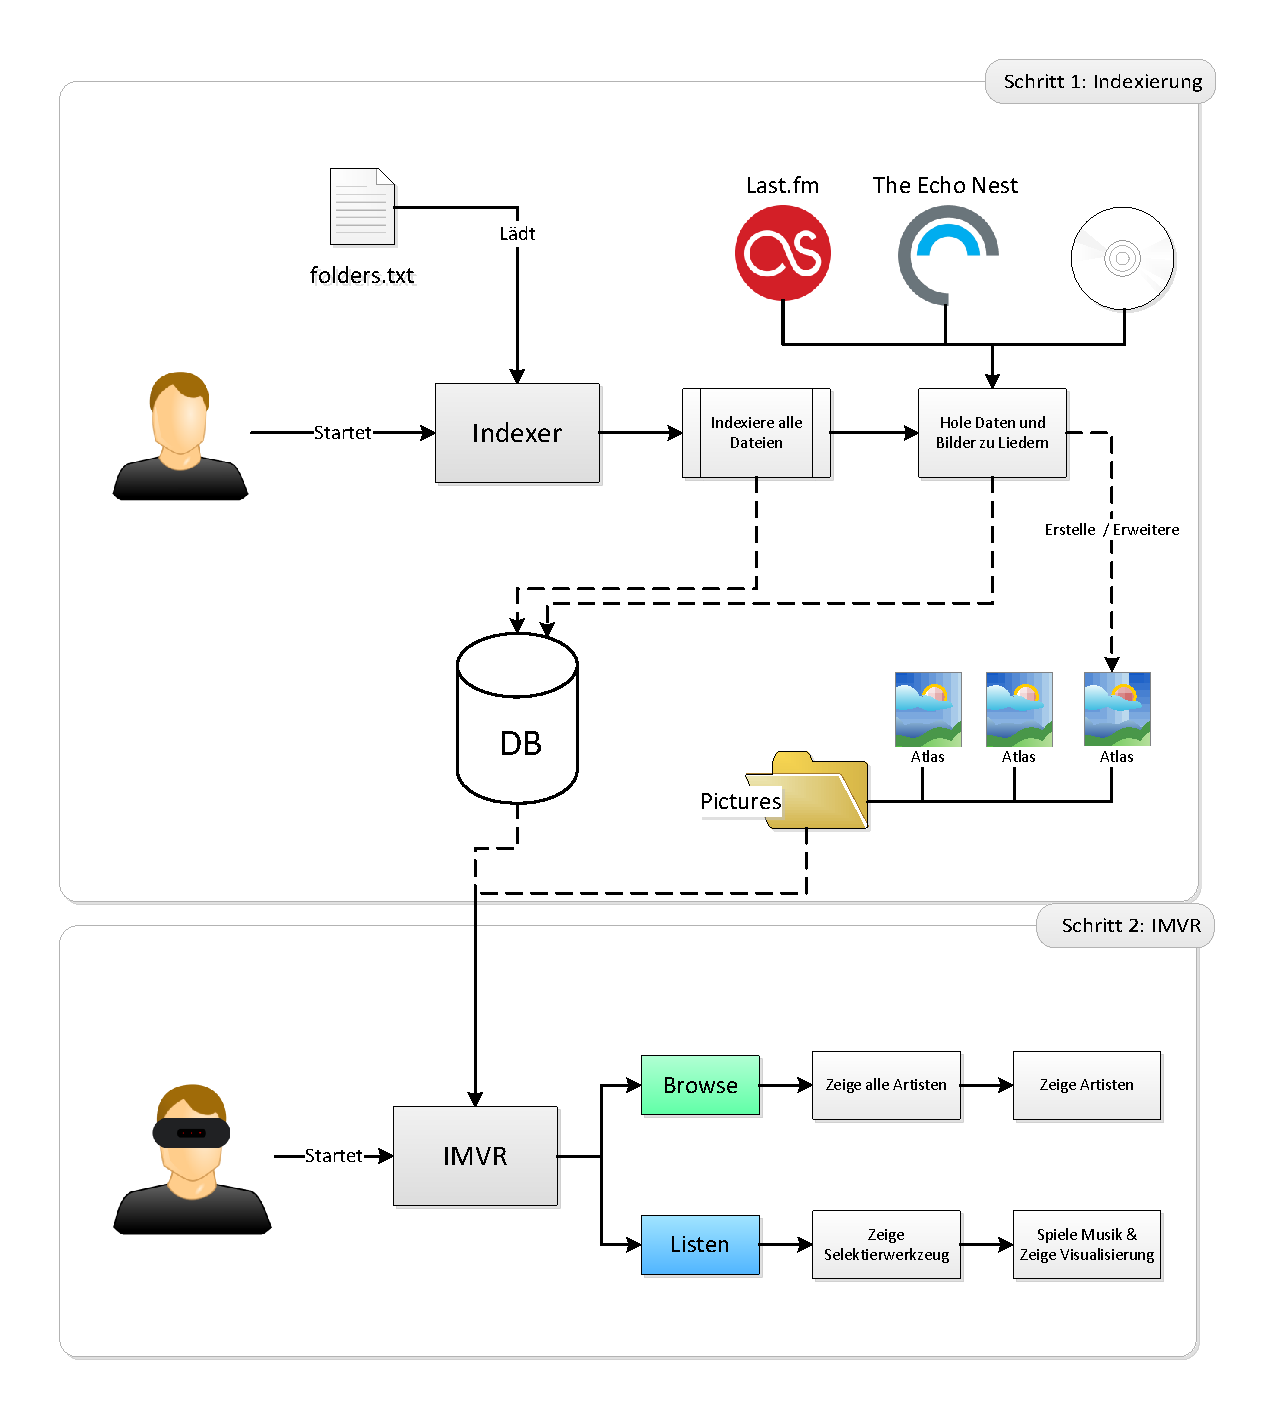
\includegraphics[width=1\linewidth]{diagramme/flow}
\caption{Grober �berblick des Programmablaufs}
\label{fig:flow}
\end{figure}

Man erkennt wie der Benutzer zuerst ausserhalb der Unity-Applikation den Indexer startet und durchlaufen l�sst. Dieser durchl�uft alle Ordner, die er in einer \textit{folders.txt} findet und schreibt diese in die Datenbank. Im n�chsten Schritt werden aus diversen Quellen weitere Daten abgerufen.

Was ebenfalls auf der Grafik zu sehen ist, sind die Atlasse. Um Ressourcen zu sparen (siehe Kapitel \ref{subsec:resources}), werden alle Bilder in sogenannten Atlassen, sprich Bildersammlungen, gespeichert. Die Bilder, von denen hier die Rede ist, sind Fotos der Artisten und das Artwork der indexierten Alben. 

Sobald die Datenbank im ersten Schritt erstellt wurde, setzt der Anwender, wie in Kapitel \ref{sec:sysoverview} beschrieben, seine Oculus Rift mit dem Leap Motion Aufsatz auf und startet IMVR. Er erh�lt dann die Auswahl, welchen Modus er beschreiten will und je nach Wahl entsprechende weitere Optionen.



\section{Systemdesign}


\chapter{Implementation des Indexers}

Ein Teil der Arbeit war es, einen Indexer zu implementieren, der die Dateien des Benutzers durchl�uft und - wie es der Name vermuten l�sst - Audiodateien indexiert. In diesem Kapitel soll auf den Aufbau und die Implementationsdetails eingegangen werden.

\section{Aufbau}

Der Indexer sowie die Datenstruktur und alle anderen Tools, die eine erg�nzende Funktion zur Hauptapplikation haben, wurden in einer separaten Visual Studio Solution zusammengefasst. In dieser befinden sich vier Projekte:

\begin{table}[H]
	\caption{Die Projekte in Auxiliary Tools}
	\centering
	\label{tab:auxiliarytools}
	\begin{tabularx}{\textwidth}{ l X }
		\toprule
		\textbf{Name} & \textbf{Beschreibung} \\ \midrule
		IMVR.Commons & DLL-Projekt, welches die Klassen enth�lt, die zwischen Applikation und Indexer geteilt werden. \\
		IMVR.Commons.Tests & Testprojekt mit Unit-Tests um die Integrit�t der Daten sicherzustellen. \\
		IMVR.Indexer & Konsolenprojekt, welches die Musikdateien auf dem Host-System indexiert. \\
		IMVR.SpeechServer & Konsolenprojekt, welches in der Vorarbeit verwendet wurde und in dieser Arbeit keine Verwendung fand. \\
		\bottomrule
	\end{tabularx}
\end{table}

Der Indexer (IMVR.Indexer) ist als parallelisiertes, knotenbasiertes System konzipiert worden. Die Parallelit�t wurde deshalb gew�hlt, weil es beim Einholen der verschiedenen Datenquellen teils zu Wartezeiten kommt, die gut anders genutzt werden k�nnen. Dieser Faktor kam besonders ins Spiel als noch zus�tzlich zu den Musikdaten auch Bilderdaten gesammelt worden sind.

Ein weiterer Grund f�r die Parallelisierung ist, dass als m�gliches Feature eine real-time Indexierung vorgesehen war, die es letztendlich allerdings nicht in das fertige Programm schaffte. Weitere Informationen zu diesem Thema werden in Abschnitt \ref{sec:indexer:herausforderungen} gegeben.


\section{Datenquellen}

Da IMVR zum Ziel hat, die Musik des Benutzers in verschiedenen Formen und Farben darzustellen, werden Daten von diversen Quellen ben�tigt. Gl�cklicherweise existiert eine grosse Datenvielfalt im Internet: Es gibt zahlreiche Online-Services, deren Gebrauch oft kostenlos ist, von denen man diverse Daten erhalten kann.

Es folgt eine kurze Zusammenstellung der untersuchten Datenquellen.

\begin{table}[H]
\caption{Eine �bersicht von verf�gbaren Online-Datenquellen.}
\centering
\label{t:datasources}
\begin{tabular}{ l l l }
	\toprule
	\textbf{Name} & \textbf{Daten} & \textbf{API-Limite} \\ \midrule
	Last.fm & Bilder, Meta-Daten & 5 Request / Sekunde \\
	The Echo Nest & Bilder, Meta-Daten, Analyse-Daten & 120 Requests / Minute \\
	Spotify & Bilder, Meta-Daten, Playlisten, Streams & ? \\
	Amazon & Bilder, Beschreibungen & 1 Request / Sekunde \\
	Gracenote & Bilder, Fingerprinting, Meta-Daten & $\sim$1000 Requests / Tag \\
	MusicBrainz & Bilder, Meta-Daten & $\sim$1 Request / Sekunde \\
	\bottomrule
\end{tabular}
\end{table}

Im Falle von IMVR kommen die Daten grunds�tzlich aus drei verschiedenen Quellen:

\begin{itemize}	
  \item ID3 Tags der Musik-Dateien
  \item The Echo Nest
  \item Last.fm
\end{itemize}

Diese wurden gew�hlt aufgrund der durchsichtigen API-Limite und den verf�gbaren Daten. The Echo Nest aggregiert zudem die Daten von anderen Stellen wie Spotify und MusicBrainz, und enth�lt wertvolle Analyse-Daten, die eine zentrale Rolle in IMVR haben.

\begin{figure}[h]
\centering
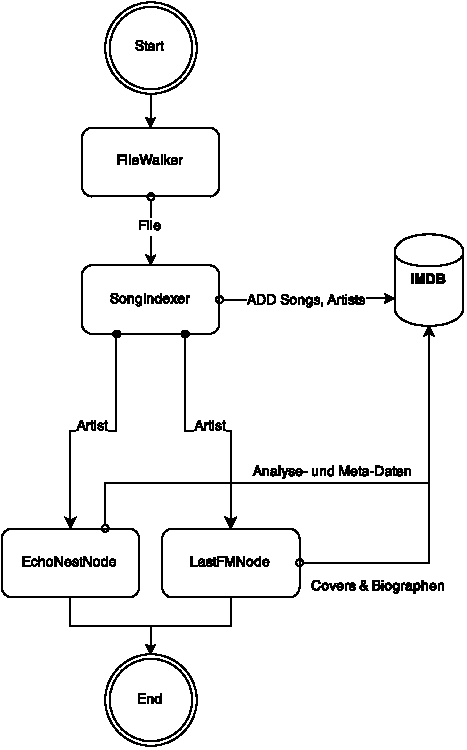
\includegraphics[width=0.5\linewidth]{bilder/Indexer-DataFlow.pdf}
\caption{Der Datenfluss, den die Files beim Indexieren nehmen.}
\label{fig:Indexer-DataFlow}
\end{figure}

In einem ersten Schritt werden grundlegende Daten wie der Titel des Liedes, der Name des Artisten, usw. aus der Datei selbst entnommen. Es wird auch gepr�ft, ob ein Album-Cover hinterlegt ist.

In einem zweiten Schritt wird �ber die .NET Bibliothek \textit{echonest-sharp} \cite{indexer:echonestcsharp}, welche im Rahmen des Projektes geforkt und erweitert wurde, zur API von The Echo Nest verbunden und diverse Meta-Daten zur Musik heruntergeladen.

Was bei der Originalimplementation leider fehlt, sind neuere Features wie Genres und Ortsdaten, sowie ein intelligenter Bremsalgorithmus, der daf�r sorgt, dass die Datenlimite eingehalten wird. Deshalb wurde ein \gls{Fork} erstellt, der diese Daten und Funktionalit�ten erg�nzt\footnote{\url{https://github.com/EusthEnoptEron/echonest-sharp/tree/additional\_apis}}.

\section{Datenstruktur}

F�r die Abspeicherung der Daten wurde zuerst ein Ansatz gew�hlt, der auf einer SQLite Datenbank basierte. Diese wurde in einem Prototyp auch erfolgreich implementiert. Es stellte sich jedoch heraus, dass diese Abh�ngigkeit das Programm unn�tig verkomplizieren w�rde und eine simple In-Memory Datenstruktur v�llig ausreicht.

Das finale Produkt verwendet also eine simple, objektorientiert Datenstruktur, die serialisiert und so zwischen den zwei Projekten (Indexer und IMVR) geteilt werden kann. Das Schema ist in Abbildung \ref{uml:IMVR.Commons} zu sehen. Damit beide Projekte Zugriff auf die genutzten Klassen haben, wurde das Schema in eine separate DLL ausgelagert, die ebenfalls als Abh�ngigkeit in beiden Projekten referenziert wird.

Anzumerken ist, dass mehrere Einstiegspunkte auf die Daten existieren und so eine gewisse Redundanz geschaffen wird. Diese Redundanz ist hilfreich, weil in IMVR mehrere Modi eben diese Einstiegspunkte ben�tigen. Aufgrund der gew�hlten Serialisierungsmethode entsteht jedoch kein grosser Speicher-Overhead.

Die Serialisierung wird durch sogenannte Protocol Buffers \cite{wiki:protobufs} realisiert, wof�r eine Open-Source Bibliothek namens \textit{protobuf-net} \footnote{\url{https://code.google.com/p/protobuf-net/}} existiert. Protocol Buffers ist ein bin�res Datenformat, welches von Google Inc. entwickelt wurde und bekannt ist f�r seine Kompaktheit und Einfachheit. Gew�hlt wurde es, weil die herk�mmliche Serialisierung mit .NETs \code{BinaryFormatter} zum Teil zu Problemen mit Unity f�hrte.

\section{Herausforderungen}
\label{sec:indexer:herausforderungen}

W�hrend der Entwicklung des Indexers kristallisierten sich diverse Schwierigkeiten heraus, welche sich grunds�tzlich in drei Kategorien einordnen lassen: organisatorische und datentechnische.

Die Organisation, oder Planung, war deshalb problematisch, weil einer der wichtigsten Faktoren f�r den Aufbau des Indexers die Vielfalt der Datentypen war. Da anfangs geplant war, Musik \textit{und} Bilder zu indexieren und darzustellen, machte eine parallele Verarbeitung der Daten Sinn und war auch notwendig.

Es wurden parallel mehrere Bilder auf mehreren CPU-Kernen analysiert, und gleichzeitig wurde auch die Musikdatenbank erweitert. Mit dem Wegfall des Bilder-Parts wird die parallele Verarbeitung also um einiges unwichtiger. Dies gilt besonders, weil bei den Metadatenquellen f�r die Musikindexierung jeweils nur ein Thread Sinn macht, da die APIs mit Limiten ausgestattet sind.

Datentechnisch stellte es sich als problematisch heraus, geeignete Datenquellen zu w�hlen, welche die notwendigen Daten simpel und mit guten API-Limiten liefern konnten. Von Anfang an war klar, dass der Service von The Echo Nest verwendet w�rde, doch dieser alleine ist nicht ausreichend. Bevor schliesslich Last.fm als Quelle f�r Album-Covers gew�hlt wurde, wurden besonders zwei APIs untersucht: Amazon und Gracenote.

Im Falle von Amazon f�hrten zwei Probleme zum Ausschluss: das Fehlen einer guten C\#-Bibliothek und die schwerf�llige Registrierung. Momentan sieht die Situation so aus, dass recht viel manuell gemacht werden muss, bzw. eine umfangreiche Service-Description importiert werden muss. \cite{indexer:amazon} In Sachen Registrierung wird erwartet, dass man eine Webseite registriert, Kontaktdaten angibt und dann gepr�ft wird.

Bei Gracenote bel�uft sich das Problem haupts�chlich auf die Daten-Limite. Diese ist nirgends �ffentlich ersichtlich, und sobald diese �berschritten wird, sind keine Requests mehr m�glich f�r den ganzen Tag. In einer Applikation wie IMVR, wo in einem Schritt alles indexiert werden soll, ist dies ein Killer-Kriterium.
\chapter{Implementation von IMVR}

Der Indexer ist implementiert und dokumentiert, also fehlt nur noch die eigentliche Applikation. Vieles hat sich im Laufe des Projekts ver�ndert und entwickelt, und viele Probleme traten zum Vorschein, die an dieser Stelle genauer erl�utert werden sollen.

\section{Unity 5}

Die Implementation von IMVR l�sst sich leider nicht ohne einen gewissen Hintergrund in Unity 5 erkl�ren. 

\subsection{Grundkonzepte}

Unity ist eine Entwicklungsumgebung und eine Spiel-Engine, die momentan aufgrund ihrer Bedienungsfreundlichkeit  und einer  frei erh�ltlichen  Version sehr  beliebt in  der Szene  der Indie-Developer ist. Gleichzeitig dient sie auch als gutes Prototyping-Tool, um schnell Ideen umzusetzen. 

Um Unity in groben Z�gen zu erkl�ren, sollen zwei Ansichtspunkte beschrieben werden: der Szenenaufbau und die Ressourcenverwaltung. 

Ein  Projekt  in  Unity  ist  in  sogenannte  \textit{Scenes}  (Szenen)  gegliedert,  welche  aus  Objekten (\textit{GameObject})  bestehen  �  das  Grundprinzip  der  Scene-Graphs  wird  also  angewandt. Speziell  ist,  dass  die  Interaktion  und  Spiellogik  grunds�tzlich  nur  innerhalb  von \textit{Components}  geschieht.  Jedes  Script  und  jede  \textit{Eigenschaft}  wird  als  Component  einem GameObject  zugeordnet.  So  hat  zum  Beispiel  ein  Licht  ein  \textit{Light}-Component  oder  die Kamera ein \textit{Camera}-Component. Selbst die Position jedes GameObjects ist nur ein Wert im  \textit{Transform}-Component.

Ein  anderer  Aspekt  von  Unity  ist  die  Ressourcenverwaltung.  Im  Grunde  genommen  ist  es 
dem  Programmierer  �berlassen,  wie  er  seine  Ressourcen  verwaltet.  Das  einzige,  was 
beachtet  werden  muss,  ist,  dass  alle  Ressourcen  im  \textit{Assets}-Folder  abgelegt  werden 
m�ssen.  �blicherweise  wird  dann  ein  Ordner  f�r  jede  Art  von  Asset  erstellt,  z.B.  f�r 
Materialien, Texturen, Meshes, Scripts, etc.

Ein  weiterer  wichtiger  Begriff  sind  die  \textit{Prefabs}.  Damit  sind  Vorlagen  gemeint,  die  man 
erstellt, indem man fertige Objekte aus der aktuellen Szene in das Asset-Folder zieht, und 
danach wiederverwerten kann. 

\subsection{Unity im Kontext von IMVR}

Was sofort auff�llt bei der Betrachtung der Ressourcenverwaltung, ist, dass diese starke Kopplung von Assets zu Projekten sich mit der grundlegenden Aufgabe dieses Projektes beisst. Unity sieht vor, dass der Programmierer w�hrend der Entwicklung alle seine Assets in den daf�r vorgesehenen Ordner platziert, das Projekt am Schluss kompiliert, und dann h�chstens im Nachhinein neue Assets als \textit{Asset Bundles} an seine Anwender verteilt. In diesem Projekt ist es jedoch zwingend n�tig, dynamisch Bilder und Musik anhand der Dateien auf dem Anwender-PC zu laden. Auf die Folgen und L�sungen zu diesem Problem wird in den Kapiteln \ref{subsec:resources} und  \ref{subsec:musicformats} n�her eingegangen.


\section{Aufbau}

\section{Darstellungskonzept}

\section{Interaktionskonzept}

Un�berraschenderweise findet die Interaktion des Users mit IMVR fast ausschliesslich mit seinen H�nden statt. In einer fr�hen Phase des Projektes war noch geplant, eventuell die Spracheingabe modal zu den H�nden zu gebrauchen, jedoch reichte daf�r die Zeit nicht mehr. Ein Artefakt dieses Vorhabens ist das \textit{SpeechServer}-Projekt, welches sich immer noch unter den \textit{AuxiliaryTools} befindet.


\subsection{Ringmen�}

Bei der Entwicklung von VR-Applikationen st�sst man zwingenderweise auf Situationen, in denen herk�mmliche Konzepte nicht mehr verwendet werden k�nnen. Die Platzierung und der Aufbau des Men�s ist so ein Punkt.

Es ist nicht leicht ein Men� korrekt zu platzieren. Eine statische Platzierung als Overlay h�lt das Interface zwar im sichtbaren Bereich, kann sich jedoch als "l�stig" herausstellen. L�sst man es verz�gert mitschweben, ger�t das Men� sofort ausser Kontrolle, und stellt man es irgendwo in die Szene und bel�sst es dabei, verliert man es sofort aus dem Blick.

Im Falle von IMVR bieten sich jedoch die H�nde als gut verwendbarer Ankerpunkt f�r das Men� an. Es gibt ein freies Projekt auf GitHub \cite{hoverVR}, welches die Finger der Hand f�r die Platzierung der Buttons in einer ringartigen Struktur verwendet. Leider befand sich das Projekt in einem zu instabilen Stadium f�r diese Arbeit, aber es lieferte die Idee f�r eine eigene, �hnliche Implementierung.

F�r IMVR wurde ebenfalls ein Ringmen� entwickelt, doch dieses verf�gt �ber keine Schaltfl�chen im herk�mmlichen Sinn. Die Finger werden auch mit Funktionen versehen, aber zum Bet�tigen benutzt der Anwender nicht seine andere Hand, sondern hebt einen Finger. Wenn ein Finger lange genug gehoben wird, wird die zugewiesene Aktion ausgef�hrt.

\subsection{Fussplatten}

Beim Erstellen einer visuellen Applikation stellt sich die Frage, wie man am besten die Struktur verdeutlichen kann. Eine Technik, die daf�r gew�hlt wurde, ist der Einsatz von "Fussplatten".

Hierbei befinden sich unter den F�ssen des Anwenders ringf�rmige Platten, welche die zwei Modi der Applikation repr�sentieren. Eine dritte, zentriert abgehobene Platte dient zur Beendigung der Applikation.

Bei diesen Platten handelt es sich um das einzige Interaktionsmittel, welches bewusst keine Eingabe durch die H�nde erfordert. In diesem Fall wird die Oculus Rift selbst als Eingabeger�t verwendet, und zwar durch den Blickwinkel.

Die Idee ist, dass der Benutzer feststellen will, ``wo er steht'', herunterschaut, und durch gehaltenen Blickkontakt mit den Fussplatten diese aktivieren kann. Entsprechend den \textit{Best Practices} wird dabei ein Indikator gef�llt, der anzeigt, wie lange der Blick noch gehalten werden muss.

Diese Art von Eingabe l�sst sich oft bei bereits erschienen Demos f�r die Oculus Rift beobachten. Das Prinzip ist sehr leicht zu implementieren und daher auch verlockend, jedoch muss mit Vorsicht vorgegangen werden: F�r den Benutzer ist es auf Dauer unangenehm, wenn von ihm st�ndige Kopfbewegungen gefordert werden. In IMVR wurde jedoch bewusst Gebrauch von dieser Methode gemacht, weil der Anwender nur selten nach unten schauen wird, und es relativ intuitiv ist.


\section{Visual Design}

\section{Herausforderungen}

\subsection{Ressourcen-Management}
\label{subsec:resources}

\subsection{Abspielen externer Musik}
\label{subsec:musicformats}

\subsection{Canvas-Elemente}

% Alpha-Sorting, etc. Tile-Blanket
\chapter{Testszenarien}

Dieses Kapitel definiert eine Reihe von Tests, mit denen das Projekt gepr�ft werden kann und soll.

\section{Indexer}

\begin{description}
	\item [T1 (Anforderung 6.1)] Der Benutzer f�gt seine ``Eigenen Bilder'' und seinen Windows-Ordner zur Library hinzu.
	\item [ $\blacktriangleright$] Der Indexer durchl�uft den Ordner fehlerfrei und die Anzahl indexierter Files, die er ausgibt, stimmt. 
	\item [T2 (Anforderung 6.2)] Der Benutzer �ffnet die Applikation.
	\item [ $\blacktriangleright$] Alle hinzugef�gten Bilder werden angezeigt und sind korrekt sortiert.
	\item [T3 (Anforderung 6.3)] Der Benutzer schliesst die Applikation und l�scht den Windows-Ordner von der Library und startet den Indexer.
	\item [ $\blacktriangleright$] Die Applikation zeigt beim n�chsten Start nur noch die Dateien im Ordner ``Eigene Bilder''.
\end{description}

\section{Bilder}

\begin{description}
	\item [$\bullet$] Der Benutzer f�gt seine ``Eigenen Bilder'' zur Library hinzu.
	\item [T1 (Anforderung 2.1)] Der Benutzer �ffnet die Applikation IMVR.
		\item [ $\blacktriangleright$] Ein 3D-Karussell (oder anders 3D-Konstrukt) mit seinen Bildern wird angezeigt.
	\item [T2 (Anforderung 2.2)] Der Benutzer �ffnet das Men� und sortiert nach Helligkeit.
		\item [ $\blacktriangleright$] Die Elemente werden neu sortiert und erscheinen geordnet nach Helligkeit.
	\item [T3 (Anforderung 2.4)] Der Benutzer ber�hrt mit den H�nden eines der Bilder.
		\item [ $\blacktriangleright$] Die �bersicht verblasst und das selektierte Bild wird vergr�ssert.
	\item [T4 (Anforderung 3.1)] Der Benutzer bewegt seine H�nde auseinander entsprechend der Gestentabelle.
		\item [ $\blacktriangleright$] Das Bild vergr�ssert sich entsprechend.
	\item [T5)] Der Benutzer wischt mit der Hand entsprechend der Gestentabelle.
		\item [ $\blacktriangleright$] Die Detailansicht wird verlassen und die �bersicht kommt wieder in den Vordergrund.
\end{description}

\section{Musik}

\begin{description}
	\item [T1 (Anforderung 4.1)] Der Benutzer f�gt seine ``Eigene Musik'' zur Library hinzu und startet den Indexer.
	\item [ $\blacktriangleright$] Alle MP3 Dateien mit korrekten ID3-Tags werden laut Log erkannt.
	\item [T2 (Anforderung 4.2)] Der Benutzer �ffnet die Applikation und wechselt in den Musikmodus.
	\item [ $\blacktriangleright$] Die soeben hinzugef�gte Musik erscheint alphabetisch geordnet.
	\item [T4 (Anforderung 1.5)] Der Benutzer �ffnet das Hauptmen� und beendet die Applikation.
		\item [ $\blacktriangleright$] Die Applikation fragt einmal nach und beendet dann.
\end{description}

\chapter{Projektmanagement}

Dieses Kapitel soll dienen, um einen organisatorischen R�ckblick auf das Projekt zu machen und die Ist-Situation mit der Soll-Situation zu vergleichen.

\section{Soll-Ist Gegen�berstellung}

In der folgenden Tabelle wird eine Gegen�berstellung des Soll-Zustands zum Ist-Zustand gemacht. Die Elemente, die sich mit der Bilderbibliothek befassten, wurden aufgrund der �nderung in der Aufgabenstellung durchstrichen und entziehen sich einer Bewertung.

\begin{longtable}{l p{0.03\textwidth} p{0.43\textwidth} p{0.43\textwidth}} \toprule %{p{0.13\textwidth} p{0.75\textwidth}} \toprule
	& \textbf{Nr.} & \textbf{Soll} & \textbf{Ist} \\ \midrule
	\endhead
	\multicolumn{4}{l}{\textbf{1. Elementares}} \\ \midrule
	\good &1.1 & Die Applikation nutzt die Oculus Rift im direkten Modus f�r die Ausgabe. &  Die Applikation nutzt die Oculus Rift im direkten Modus f�r die Ausgabe. \\
	\good &1.2 & Die Applikation ist vollst�ndig mit den H�nden bedienbar. & Die Applikation ist vollst�ndig mit den H�nden bedienbar, verwendet jedoch den Blick also weitere Eingabem�glichkeit. \\
	\good &1.3 & Die Applikation erlaubt den Zugriff auf alle gefundenen, validen Dateien. & Die Applikation erlaubt den Zugriff auf alle gefundenen, validen Dateien. \\
	\good &1.4 & Bilder k�nnen angeschaut werden, Musik kann angeh�rt werden. & Musik kann angeh�rt werden und relevante Bilder k�nnen angeschaut werden. \\
	\good &1.5 & Die Applikation kann jederzeit beendet werden. & Die Applikation kann per Blick auf die entsprechende Fussplatte jederzeit beendet werden. \\
	\meh &1.6 & Die Applikation erreicht eine stetige Framerate von mindestens 60fps auf dem Referenzsystem\footnote{Intel(R) Xeon CPU E5-1650 v3 @ 2.50Ghz mit 32GB RAM und einer NVIDIA GeForce GTX 980 Grafikkarte.}. & Es gibt noch Einbr�che in der Framerate bei Szenenwechsel. \\
	\meh &1.7 & Die Applikation kann min. 100'000 Dateien verarbeiten. & Das Anzeigen in der �bersicht wird aufgrund von Vertices-Beschr�nkungen problematisch. Hinzuf�gen von 100\,000 Elementen zur Playlist ist jedoch m�glich.\\
	\good &1.8 & H�nde werden abstrakt dargestellt. & H�nde werden abstrakt mithilfe von Partikeln dargestellt. \\
	\good &1.9 & Die Hintergrundmusik kann von der Musikbibliothek ausgew�hlt werden. & Die Hintergrundmusik kann von der Musikbibliothek ausgew�hlt werden. \\
	\multicolumn{4}{l}{\textbf{\sout{2. �bersicht (Bilder)}}} \\ \nopagebreak \midrule
	\multicolumn{4}{l}{\textbf{\sout{3. Detailansicht (Bilder)}}} \\ \nopagebreak \midrule
	\multicolumn{4}{l}{\textbf{4. �bersicht (Musik)}} \\ \nopagebreak \midrule
	\good &4.1 & Unterst�tzt mit ID3-Tags versehene MP3. & Unterst�tzt mit ID3-Tags versehene MP3. \\
	\good &4.2 & Dateien werden alphabetisch gruppiert nach Artisten dargestellt. & Dateien werden im Browse-Modus alphabetisch gruppiert nach Artisten dargestellt. \\
	\bad &4.3 & Dateien k�nnen nach Album, Genre und Jahr gruppiert werden & Eine Gruppierfunktion wird momentan nicht unterst�tzt. \\
	\meh &4.4 & Alben k�nnen anhand ihres Covers wie Bilder dargestellt werden. & Alben werden in der Detailansicht mit einem Cover dargestellt. \\
	\good &4.5 & Unterst�tzt weitere Musikformate (Ogg Vorbis, FLAC, M4A, APE, TAK, etc.) & Alle von CSCore \cite{cscore} unterst�tzten Formate sind abspielbar\footnote{MP3, WAVE, FLAC, AAC, AC-3, WMA, Ogg Vorbis}. \\
	\meh &4.6 & Dateien k�nnen ungruppiert dargestellt werden. & Im Listen-Modus werden Songs unabh�ngig des K�nstlers oder des Albums betrachtet.\\
	\multicolumn{4}{l}{\textbf{5. Detailansicht (Musik)}} \\ \midrule
	\good &5.1 & Album mit einer Liste von Liedern wird dargestellt. & Album mit einer Liste von Liedern wird dargestellt. \\
	\good &5.2 & Eine Datei kann zur Wiedergabe ausgew�hlt werden. & Eine Datei kann zur Wiedergabe ausgew�hlt werden. \\
	\good &5.3 & Die Wiedergabe wird visuell untermalt (Spektrogramm). & Es gibt diverse visuelle Effekte zur Untermalung der Musik. \\
	\meh &5.4 & Informationen zum Artisten werden dargestellt (Ort, Beschreibung, Gr�ndungsjahr) & Die Daten sind vorhanden, aber es werden noch nicht alle dargestellt. \\
	\multicolumn{4}{l}{\textbf{6. Indexierung}} \\ \nopagebreak \midrule
	\good &6.1 & Der Benutzer kann einen oder mehrere Ordner angeben, die nach Bilder und Musik gescannt werden. & Der Benutzer kann einen oder mehrere Ordner angeben, die nach Bilder und Musik gescannt werden. \\
	\good &6.2 & Die gefundenen Dateien werden mit diversen Kennwerten indexiert. & Die gefundenen Dateien werden mit diversen Kennwerten indexiert. \\
	\good &6.3 & Dateien, die nicht mehr in einem der Medienordner liegen, werden aus dem Index gel�scht. & Dateien, die nicht mehr in einem der Medienordner liegen, werden aus dem Index gel�scht. \\
	\bad &6.4 & Die indexierten Ordner k�nnen innerhalb der Applikation angegeben werden & Die Indexierung ist vollst�ndig getrennt von IMVR.\\
	\bad &6.5 & Die Indexierung kann innerhalb der Applikation durchgef�hrt werden. & Die Indexierung wird vorher und f�r sich durchgef�hrt.\\
	\multicolumn{4}{l}{\textbf{7. Sonstige Funktionen}} \\ \midrule
	\meh & 7.1 & Es k�nnen Filter �ber die Musik gelegt werden (Low-Pass, High-Pass, Compressor, etc.) & Momentan werden keine Filter unterst�tzt, die Musik ist jedoch in einem Mixer eingebunden und f�r Filtereffekte vorbereitet.\\
	&\sout{7.2} & \sout{Bildergruppen k�nnen als ``Diashow'' angeschaut werden.} & \\
	\bad & 7.3 & Es ist eine Netzwerkfunktion vorhanden, die es erlaubt, die Fotosammlung zu zweit anzuschauen. & Es werden keine Netzwerkfunktionen angeboten. \\
	\meh &7.4 & Gesamtstatistiken k�nnen angezeigt werden (Bildalter / Anzahl, Aufl�sung / Anzahl, Aufl�sung / Anzahl, Kartenchart mit Anzahl Fotos) & Es sind ein paar Statistiken zu Metadaten im System vorhanden. \\
	\bad &7.5 & Online-Services k�nnen als Datenquelle angegeben werden (Flickr, Spotify, etc.) & Es werden keine dynamischen Online-Services unterst�tzt.\\
	\caption{Eine Gegen�berstellung der Soll-Kriterien mit dem Ist-Zustand}
	\label{tab:pflichten}
\end{longtable}

\begin{landscape}
	\section{Zeitplan}
	\begin{figure}[H]
		\centering
		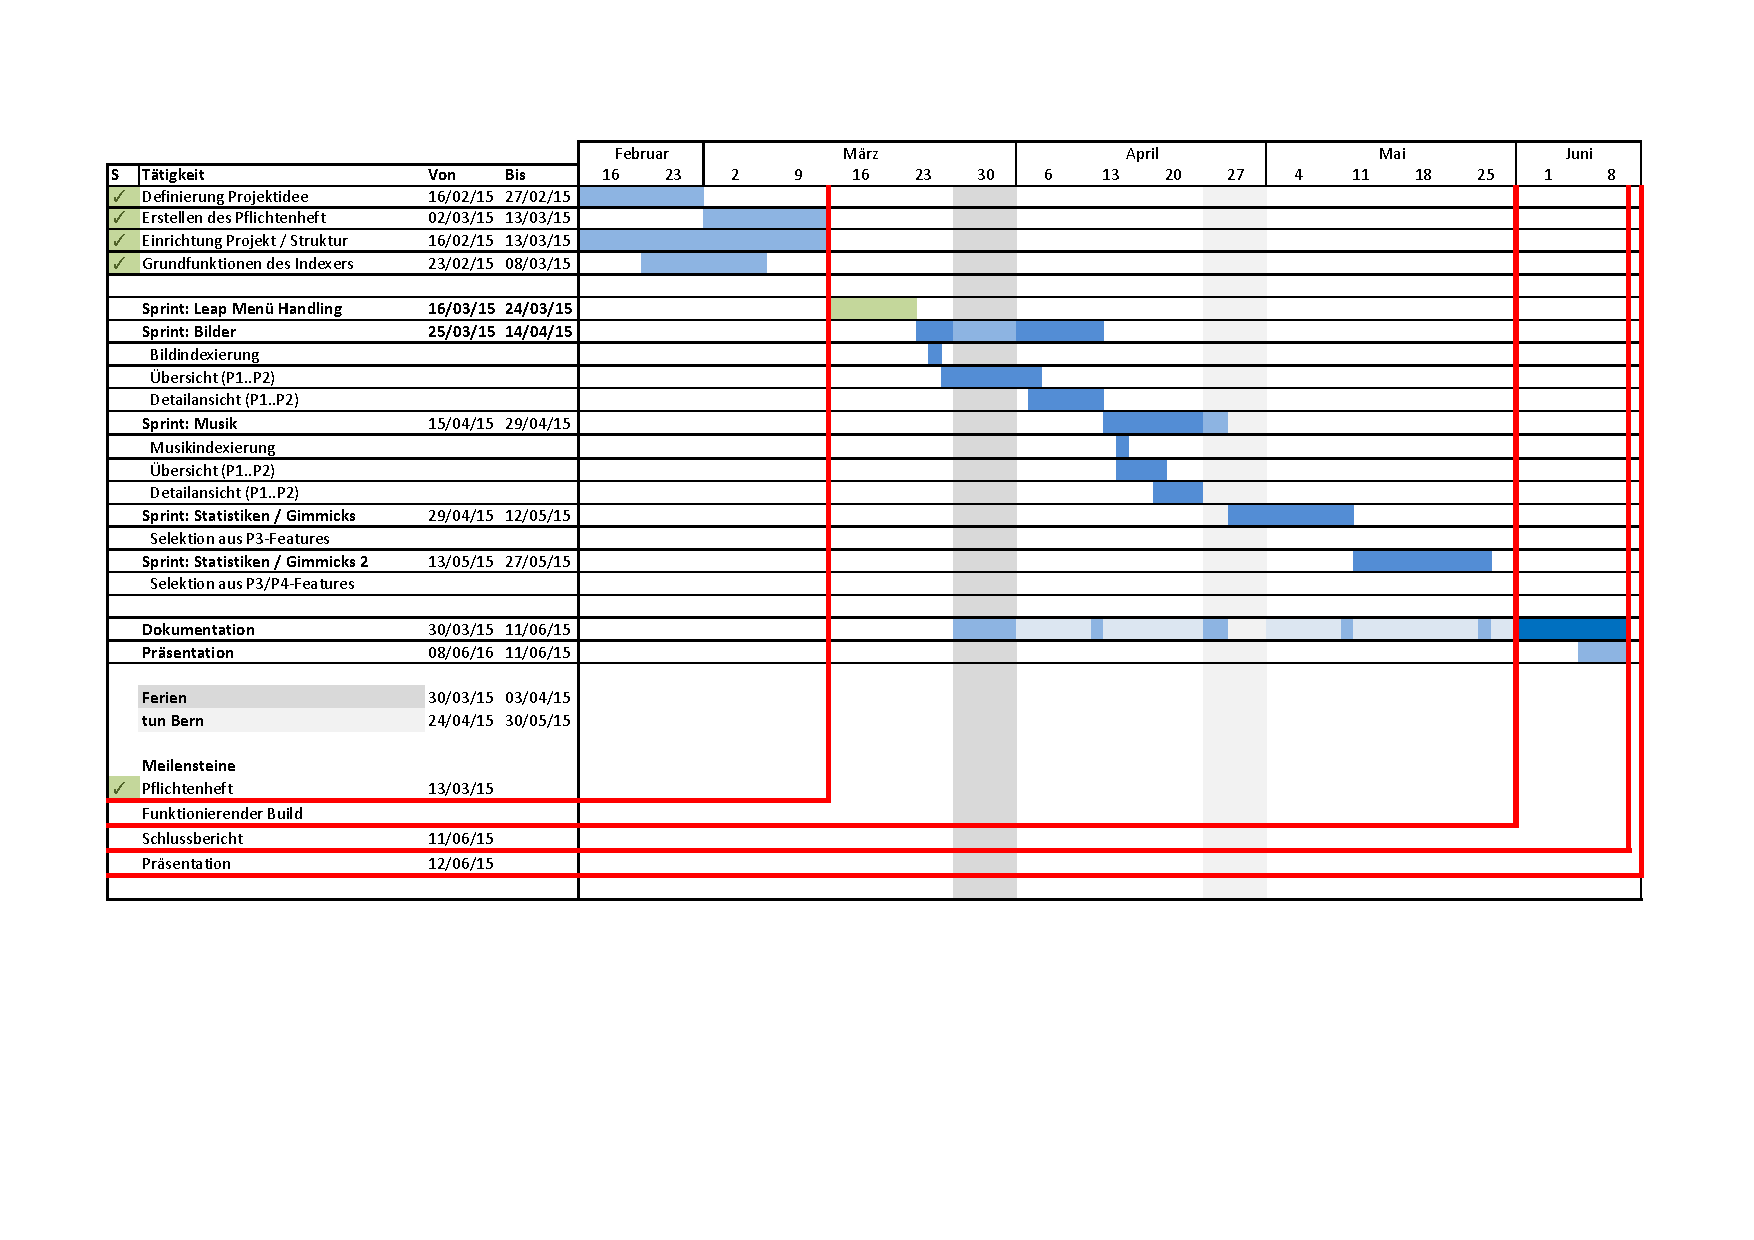
\includegraphics[trim=10mm 55mm 10mm 20mm, clip=true, width=1.1\linewidth]{../Zeitplan/Zeitplan}
		\caption{Der Zeitplan mit Sprints und Priorit�ten.}
	\end{figure}
	
\end{landscape}
\chapter{Schlussbetrachtung}

Zum Schluss soll kurz ein Blick auf die Gegenwart, die Vergangenheit und die Zukunft geworfen werden. War das Projekt erfolgreich? Wo lagen die \textit{Pitfalls}? Wie geht es weiter? Diese Fragen sollen an dieser Stelle beantwortet werden. 

\section{Ergebnis}



\section{Reflexion}

Grunds�tzlich ist das Ergebnis zufriedenstellend ausgefallen. Es gibt allerdings zahlreiche Punkte, welche besser h�tten gel�st werden k�nnen.

Aufgrund der experimentellen Natur des Projektes war die Planung teilweise nicht so ausgearbeitet und zuverl�ssig, wie sie es in einem herk�mmlichen Projekt w�re. Durch das Ver�ndern von Funktionalit�t, dem wiederholten Refactoring, und der ge�nderten Zielsetzung entstand zum Teil zus�tzliche Komplexit�t und zu einem gewissen Masse auch ``Code-Smell'' \cite{wiki:codesmell}.

Eine Lektion, die ebenfalls gelernt wurde, ist, dass Computergrafik unberechenbar sein kann und viele T�cken bereith�lt. Mehrmals vergingen Stunden, bis die Ursache eines Bugs oder einer fehlerhaften Funktion herausgefunden werden konnten, gefolgt von zahlreichen Stunden, die zur Behebung aufgewendet werden mussten.

Im Nachhinein kann auch gesagt werden, dass Unity nicht die ideale Wahl f�r die Umsetzung der Projektidee war. Die Umgebung ist zu sehr um Assets und die Idee von geschlossenen Spielen aufgebaut, und eignet sich nicht sehr gut f�r dynamische Inhalte. Eventuell h�tte die Unreal Engine 4 \cite{ue4} in dieser Hinsicht bessere Resultate geliefert. Es muss allerdings auch gesagt werden, dass eine Einarbeit in die Unreal Engine in Hinsicht auf das Vorprojekt keinen Sinn gemacht h�tte und somit keine grosse Wahl bestand.

Nichtsdestotrotz bzw. eben aufgrund der zahlreichen H�rden erlaubte die Entwicklung von IMVR einen Einblick in viele Features und Eigenheiten von Unity und fiel somit sehr informativ und lehrreich aus. Meshes wurden generiert, ein eigenes Input Modul wurde geschrieben, das UI wurde erforscht und die Grenzen und Asset-Gebundenheit wurde erkannt.

Eine nicht ganz so offensichtliche Kompetenz, die ebenfalls im Verlaufe des Projektes angeeignet und verbessert werden konnte, ist der Umgang von grossen Projekten mit Git bzw. GitHub. Die Ordnerstruktur war zwar von Beginn an geplant,  wurde jedoch w�hrend des Projekts erweitert und optimiert. Die Verwendung eines \gls{vcs} erwies sich allgemein als n�tzlich, wenn kurz etwas getestet werden sollte oder bei Vergleichen mit �lteren Revisionen, wenn ein Feature nicht mehr funktionierte.

Ich kann also abschliessend sagen, dass ich mir dank des Projektes eine solide Basis an Fachwissen in Unity und Computergrafik aneignen konnte, und das Projekt somit als Erfolg betrachte.

\section{Ausblick}

Die Grundfunktionalit�t von IMVR ist zwar implementiert, es bleibt jedoch noch viel Raum f�r Verbesserungen und Erweiterungen. Es gibt mehrere Richtungen, in die sich das Tool weiterentwickeln k�nnte.

Eine M�glichkeit w�re die simple Erweiterung der Funktionalit�t in die Breite. Damit ist gemeint, dass weitere Ansichten auf die Daten implementiert werden k�nnten. Momentan ist es nur m�glich, alle K�nstler auf dem lokalen System in einer Zylinderstruktur darzustellen, aber nichts spr�che dagegen, dasselbe f�r die Alben oder Lieder zu machen. Ebenfalls m�glich w�ren Sortier- und Gruppierfunktionen, wie anfangs geplant war.

Anders gesehen, k�nnte man die Applikation auch noch weiter in die Tiefe entwickeln. Seit Fr�hjahr 2015 bietet Oculus Rift ein Audio SDK an, welches 3D-Sound mit Stereokopfh�rer simulieren kann. Erste eigene Tests f�hrten zum Schluss, dass die Implementierung viel umfangreicher und robuster ist, als Unitys eingebauter 3D-Sound. Es g�be sicher ein paar interessante Einsatzgebiete f�r dieses Feature.

Weiterhin k�nnte man auch noch weitere Metadaten hinzuziehen oder die vorhandenen besser auswerten. Verschiedene Web-Services bieten verschiedene Arten von Daten an, die miteinander kombiniert werden k�nnten, um neue Schl�sse zu ziehen. W�hrend des Projektes kam beispielsweise die Idee auf, Selektionen von Metadatenbereichen als selbst definierbare ``Presets'' abzuspeichern, damit eine leichtere  und aussagekr�ftigere Suche m�glich w�re.

Auch der Weg zur vollumfangreichen Mediacenter-L�sung st�nde offen. W�rde man die Bilderbibliothek wieder hinzunehmen, w�re bereits der erste Schritt getan. Die Einbindung von Videodaten w�rde aufgrund der Limitierungen von Unity jedoch problematisch werden. Jedoch w�re auch dieses Problem keineswegs undurchf�hrbar - zumal es im Asset Store bereits passende Plugins gibt.





%\chapter{Einleitung}
\label{chap:einleitung}

Der Markt der stereoskopischen Brillen befindet sich in einem starken Wachstum. Oculus Rift, SteamVR, Project Morpheus, Nvidia VR - die Liste der teilnehmenden Partien w�chst und w�chst, doch neue Ausgabeger�te ben�tigen auch neue Eingabeger�te. Die Leap Motion kann als ein solches gez�hlt werden und bietet eine freie Handerkennung ohne irgendwelche Handschuhe tragen zu m�ssen.

In diesem Projekt geht es darum, die neuartige Eingabem�glichkeiten der Leap Motion in Verbindung mit der Oculus Rift einzusetzen und damit eine interaktive \gls{vr}-Applikation zu schreiben. Im Rahmen eines vorhergehenden Projekts wurde die Materie bereits bearbeitet und die M�glichkeiten erforscht. Es geht nun also haupts�chlich um die erfolgreiche Anwendung der erarbeiteten Informationen.
%\chapter{Vision ``IMVR''}

Die Vision soll dazu dienen, einen �berblick �ber die Applikation zu geben, die im Rahmen der Bachelorarbeit erstellt wird.

\section{Problemstellung}

Es soll eine Applikation namens ``\gls{imvr}'' entwickelt werden, welche Gebrauch von der Oculus Rift macht, um die Bilder- und Musiksammlung des Anwenders ansprechend darzustellen, z.B. in Form eines 3D-Karussels. Die zus�tzliche "Tiefe", die durch den Einsatz eines stereoskopischen \gls{hmd} entsteht, soll dem Anwender helfen, sich in seiner Medienbibliothek schneller zurechtzufinden.

Zus�tzlich dazu soll die Leap Motion dazu verwendet werden, um vollst�ndige Handfreiheit zu gew�hren: Der Anwender soll komplett ohne Maus und Tastatur imstande sein, sich durch seine Bilder zu navigieren.

Kurz zusammengefasst muss die Applikation:

\begin{itemize}
	\item Die Bild- und Musikbibliothek des Benutzers in stereoskopischem 3D darstellen.
	\item Diese freih�ndig durchsuchbar machen mit Sortier- und evtl. Gruppierfunktion.
	\item Die Bilder betrachtbar und die Musik abspielbar machen.
	\item Metainformationen darstellen (z.B. in Form von Diagrammen).
\end{itemize}

Zus�tzlich zur Applikation selbst soll noch ein zus�tzliches Tool entwickelt werden, welches im Voraus die Dateien auf dem Host-System indexiert und f�r die visuelle Applikation bereitstellt.

\section{Technologien}

Das Projekt verwendet spezielle Hardware und Software. Es folgt eine kurze Erkl�rung zu diesen Technologien.

\subsection{Oculus Rift}

Die Oculus Rift ist ein stereoskopisches \gls{hmd}, welches durch Oculus VR entwickelt wird. Die aktuelle Version ist das Developer Kit 2 (DK2). Ein Termin f�r die finale Version steht noch nicht fest.

Hardwarem�ssig besteht die Rift aus einem Headset f�r das Bild und einer Kamera f�r das Head-Tracking. Das Headset wird per USB und HDMI an den Computer angeschlossen und �ber ein Stromkabel mit Strom versorgt. Die Kamera wird auf dem Computerbildschirm platziert, und per USB an den Computer und per Sync-Kabel an die Rift angeschlossen.

\begin{figure}[h]
\centering
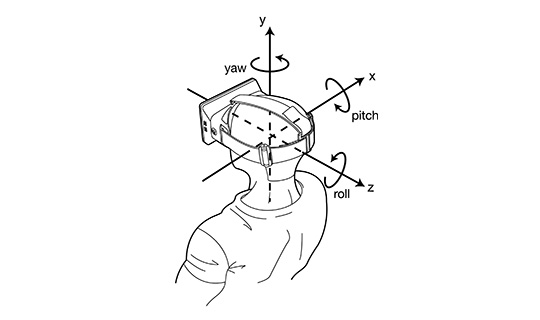
\includegraphics[width=0.7\linewidth]{bilder/rift1}
\caption{Illustration, welche die Anwendung und das Koordinatensystem der Oculus Rift verdeutlicht.}
\floatfoot{Quelle: \url{https://www.oculus.com/blog/building-a-sensor-for-low-latency-vr/}}
\label{fig:rift1}
\end{figure}

Seit DK2 ist das Headset mit 40 Infrarot-LEDs best�ckt, welche mit einer bestimmten Frequenz aufleuchten und von der Kamera f�r das Head-Tracking benutzt werden.
 
Auf der Software-Seite wird ein Treiber auf dem Computer installiert, der nach einer Registration als Entwickler auf der offiziellen Seite erh�ltlich ist . Die Software erlaubt die Erstellung von Benutzerprofilen, um die \gls{ipd} korrekt einzustellen. Es ist ausserdem m�glich, zwischen zwei Betriebsmodi auszuw�hlen: dem traditionellen Modus, wo die Rift als zweiter Bildschirm angesprochen wird, und dem neuen ``Direct Mode'', wo die Rift direkt angesprochen wird.

\subsection{Leap Motion}

Die \gls{leap} besteht aus einem rechteckigen Ger�t mit zwei Infrarotsensoren, welche deren Daten per USB auf den angeschlossenen Computer �bertr�gt. Nach der Installation der Leap Motion Runtime l�uft auf dem Computer ein Service, der diese Daten empf�ngt, verarbeitet und per API mit einer variablen Framerate verschiedenen Applikationen zur Verf�gung stellt.

Die Daten, welche diese API liefert, sind in sogenannte ``Frames'' gruppiert. Ein Frame ist sozusagen eine Momentaufnahme der Realit�t, welche sich aus erkannten H�nden zusammensetzt. Durchschnittlich werden pro Sekunde etwa um die 100 dieser Frames berechnet.

\begin{figure}[H]
	\centering
	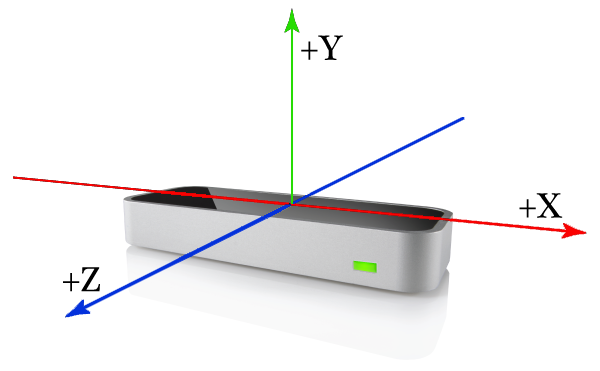
\includegraphics[width=0.7\linewidth]{bilder/leap1}
	\caption{Verdeutlichung des Koordinatensystems.}
	\floatfoot{Quelle: \url{https://developer.leapmotion.com/documentation/csharp/devguide/Leap_Coordinate_Mapping.html}}
	\label{fig:leap1}
\end{figure}

Durch diese Frames kann man auf die Daten der H�nde zugreifen. Jede Hand erh�lt eine ID, womit man gleiche H�nde Frame-�bergreifend identifizieren kann, sowie die dazugeh�renden Koordinaten und Drehungen. Auf Abbildung \ref{fig:leap1} wird ersichtlich, dass sich die Koordinaten in einem rechtsh�ndigen Koordinatensystem befinden, wobei die Y-Achse nach oben zeigt und die Masse in Millimeter angegeben sind. Die Koordinaten der Finger sind innerhalb von Finger-Instanzen gruppiert, welche wiederum ihre Gelenke als Instanzen einer Joint-Klasse zur Verf�gung stellen.

\begin{figure}[H]
	\centering
	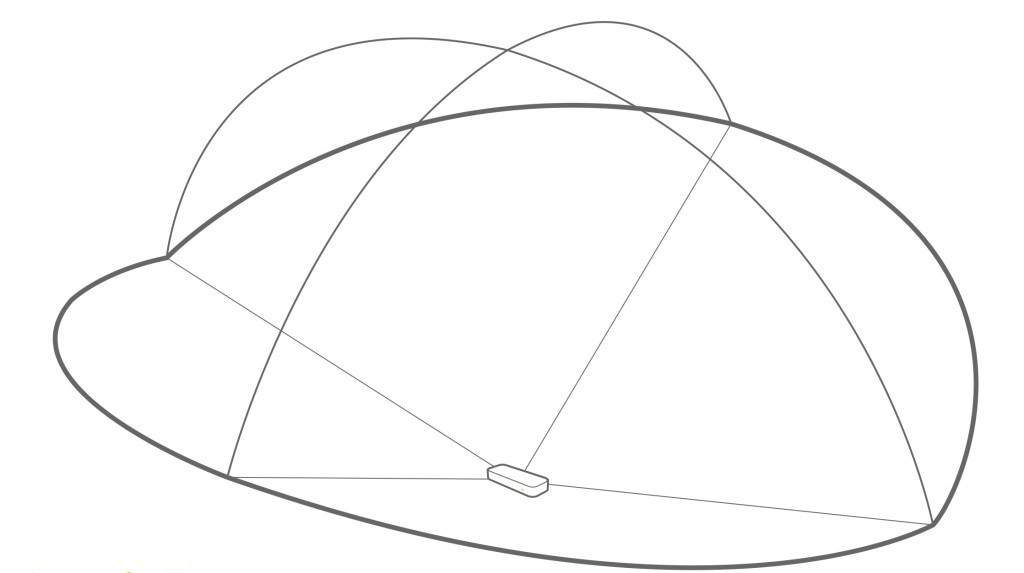
\includegraphics[width=0.7\linewidth]{bilder/leap2}
	\caption{Das Sichtfeld der Leap Motion.}
	\floatfoot{Quelle: \url{https://community.leapmotion.com/t/accurately-measuring-distances/842/3 }}
	\label{fig:leap2}
\end{figure}

Die Leap Motion hat ungef�hr eine Reichweite von einem Meter, wobei das Interaktionsfeld einer Form, wie in Abbildung \ref{fig:leap2} ersichtlich ist, entspricht. Das Sichtfeld liegt bei 150� in vertikaler und 120� in horizontaler Richtung.


\subsection{Unity 5}

\gls{unity} ist eine Entwicklungsumgebung und eine Spiel-Engine, die momentan aufgrund ihrer Bedienungsfreundlichkeit und einer frei erh�ltlichen Version sehr beliebt in der Szene der Indie-Developer ist. Gleichzeitig dient sie auch als gutes Prototyping-Tool, um schnell Ideen umzusetzen.

Am 3. M�rz 2015 machte Unity einen Versionssprung und ist nun unter dem Namen ``Unity 5'' erh�ltlich. Neben anderen Neuerungen sind jetzt alle Funktionen, f�r die fr�her eine kostenpflichtige Lizenz erworben werden musste, auch in der freien Version erh�ltlich, was f�r dieses Projekt einen gr�sseren Spielraum bedeutet.

In diesem Projekt wurde Unity wegen der angenehmen Lernkurve und der guten Integrierung mit der Oculus Rift und der Leap Motion f�r den Einsatz gew�hlt. Wie bereits erw�hnt wurde, ist es leicht, schnell zu Ergebnissen zu kommen, und die Entwicklungsumgebung unterst�tzt die zwei Programmiersprachen, die der Verfasser dieses Dokuments am besten beherrscht.

\section{Anwendung}

Innerhalb von \gls{imvr} wird die Leap Motion mit einer Halterung an der Oculus Rift befestigt, welche auf der offiziellen Website von Leap Motion f�r rund \$15\footnote{Siehe \url{https://www.leapmotion.com/product/vr}} erh�ltlich ist. Wie in Abbildung \ref{fig:uebersicht} ersichtlich ist, sind beide Ger�te unter Anderem per USB am PC befestigt und senden dar�ber ihre Daten an die entsprechenden Services. Diese leiten wiederum die ausgewerteten Daten durch �ffentliche APIs an Unity bzw. IMVR weiter.

\afterpage {
\begin{figure}[t!]
	\centering
	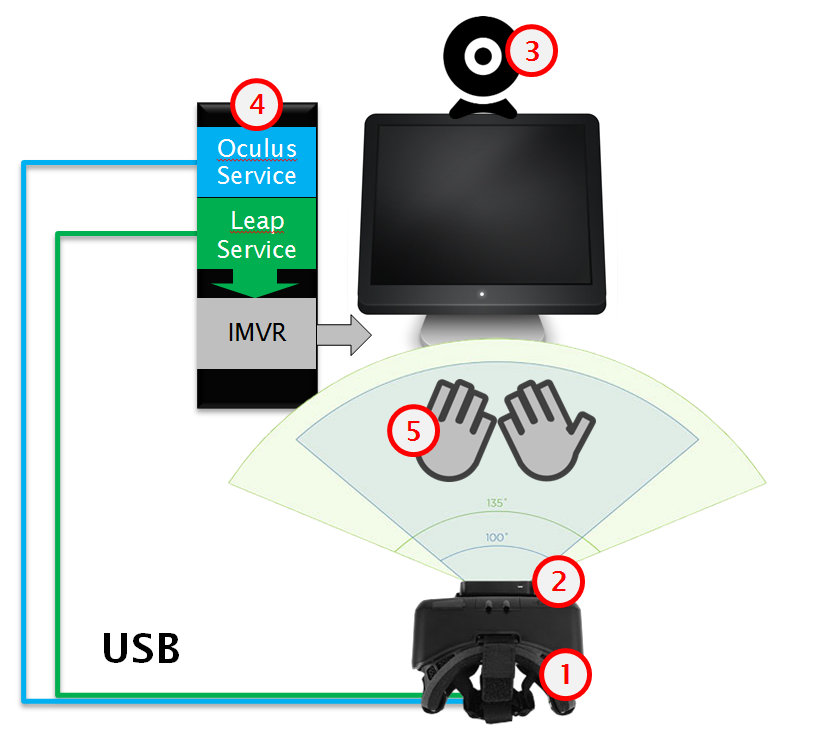
\includegraphics[width=0.8\linewidth]{bilder/systemuebersicht}
	\caption{Eine �bersicht der Technologien und wie sie verbunden sind.}
	\label{fig:uebersicht}
\end{figure}

\begin{table}[H]
	\centering
	\begin{tabular}{p{0.1\linewidth} p{0.3\linewidth} p{0.5\linewidth}}
		\textbf{Nr.} & \textbf{Komponente} & \textbf{Beschreibung} \\ \midrule
		1. & Oculus Rift DK2 & \gls{hmd} f�r den grafischen Output. \\
		2. & Leap Motion & Ger�t, welches H�nde erkennt und ihre Koordinaten an den Computer sendet. \\
		3. & Oculus Rift Kamera & Kamera, welche seit dem DK2 f�r das �rtliche Tracking zust�ndig ist. \\
		4. & Computer & Host-System f�r IMVR. \\
		5. & Benutzer & Benutzer, der die Oculus Rift tr�gt und mit seinen H�nden das Programm steuert. \\
	\end{tabular}
\end{table}
}

\clearpage
%\chapter{Spezifikationen}

In diesem Kapitel sollen die Anforderungen, die in der Vision grob geschildert wurden, konkretisiert und aufgelistet werden.

\section{Funktionale Anforderungen}

In der folgenden Tabelle sind alle Anforderungen aufgelistet mit einer Priorit�t von 1 bis 5, wobei eine tiefere Zahl f�r eine h�here Priorit�t steht. Grunds�tzlich kann gesagt werden, dass alle Anforderungen, die mit einer 1 deklariert werden, implementiert werden m�ssen und alle Anforderungen, die mit einer 5 deklariert werden, nur Ideen sind, welche mit hoher Wahrscheinlichkeit nicht implementiert werden k�nnen.

%\begin{table}[H]
	\begin{longtable}{p{0.06\textwidth} p{0.7\textwidth} p{0.13\textwidth}} \toprule %{p{0.13\textwidth} p{0.75\textwidth}} \toprule
		\textbf{Nr.} & \textbf{Beschreibung} & \textbf{Priorit�t} \\ \midrule
		\endhead
		\multicolumn{3}{l}{\textbf{1. Elementares}} \\ \midrule
		1.1 & Die Applikation nutzt die Oculus Rift im direkten Modus f�r die Ausgabe. & 1 \\
		1.2 & Die Applikation ist vollst�ndig mit den H�nden bedienbar. & 1 \\
		1.3 & Die Applikation erlaubt den Zugriff auf alle gefundenen, validen Dateien. & 1 \\
		1.4 & Bilder k�nnen angeschaut werden, Musik kann angeh�rt werden. & 1 \\
		1.5 & Die Hintergrundmusik kann von der Musikbibliothek ausgew�hlt werden. & 2 \\
		1.6 & Die Applikation kann jederzeit beendet werden. & 1 \\
		1.7 & H�nde werden abstrakt dargestellt. & 2 \\
		1.8 & Die Applikation erreicht eine stetige Framerate von mindestens 60fps auf dem Referenzsystem\footnote{Intel(R) Xeon CPU E5-1650 v3 @ 2.50Ghz mit 32GB RAM und einer NVIDIA GeForce GTX 980 Grafikkarte.}. & 1 \\
		\multicolumn{3}{l}{\textbf{2. �bersicht (Bilder)}} \\ \nopagebreak \midrule
		2.1 & Elemente k�nnen in einem 3D-Karussell dargestellt werden. & 1 \\
		2.2 & Elemente k�nnen selektiert werden. & 2 \\
		2.3 & Elemente k�nnen getaggt werden. & 3 \\
		2.4 & Es kann auf ein bestimmtes Element fokussiert werden (siehe Detailansicht). & 1 \\
		2.5 & Es ist eine Mehrfachselektierung m�glich. & 3 \\
		2.6 & Elemente k�nnen in anderen Anordnungen dargestellt werden (Tunnel, Fluss, Fl�che, W�rfel, etc.) & 3 \\
		2.7 & Bilder k�nnen nach Farbton, S�ttigung und Helligkeit sortiert werden. & 1 \\
		2.8 & Bilder k�nnen alphabetisch und chronologisch sortiert werden. & 2 \\
		2.9 & Bilder k�nnen nach Dateiordner gruppiert werden. & 3 \\
		2.10& Bilder k�nnen nach Kennwerten (Varianz, Entropie) sortiert werden & 3 \\
		\multicolumn{3}{l}{\textbf{3. Detailansicht (Bilder)}} \\ \nopagebreak \midrule
		3.1 & Bild kann vergr�ssert und verkleinert werden. & 1 \\
		3.2 & Bild kann gel�scht werden & 2 \\
		3.3 & Ein (3D)-Histogramm des Bildes wird angezeigt. & 3 \\
		3.4 & Die Metadaten von Fotos werden dargestellt & 4 \\
		3.5 & Der Hintergrund passt sich den Metadaten entsprechend an & 5 \\
		3.6 & Es k�nnen zus�tzliche Versionen des Bildes (inkl. Histogram) angezeigt werden und mit Punktoperationen ver�ndert werden. & 4 \\
		3.7 & Die zus�tzlichen Bilder k�nnen auch mit lokalen und globalen Operationen gefiltert werden. & 5 \\
		\multicolumn{3}{l}{\textbf{4. �bersicht (Musik)}} \\ \nopagebreak \midrule
		4.1 & Unterst�tzt MP3 und WAVE. & 1 \\
		4.2 & Unterst�tzt weitere Musikformate (Ogg Vorbis, FLAC, M4A, APE, TAK, etc.) & 5 \\
		4.3 & Dateien werden alphabetisch gruppiert nach Artisten dargestellt & 1 \\
		4.4 & Dateien k�nnen nach Album, Genre und Jahr gruppiert werden & 3 \\
		4.5 & Dateien k�nnen ungruppiert dargestellt werden. & 5 \\
		4.6 & Alben k�nnen anhand ihres Covers wie Bilder dargestellt werden. & 3 \\
		\multicolumn{3}{l}{\textbf{5. Detailansicht (Musik)}} \\ \midrule
		5.1 & Album mit einer Liste von Liedern wird dargestellt. & 1 \\
		5.2 & Eine Datei kann zur Wiedergabe ausgew�hlt werden. & 1 \\
		5.3 & Die Wiedergabe wird visuell untermalt (Spektrogramm). & 2 \\
		5.4 & Informationen zum Artisten werden dargestellt (Ort, Beschreibung, Gr�ndungsjahr) & 3 \\
		\multicolumn{3}{l}{\textbf{6. Indexierung}} \\ \nopagebreak \midrule
		6.1 & Der Benutzer kann einen oder mehrere Ordner angeben, die nach Bilder und Musik gescannt werden. & 1 \\
		6.2 & Die gefundenen Dateien werden mit diversen Kennwerten indexiert. & 1 \\
		6.3 & Die Indexierung kann innerhalb der Applikation durchgef�hrt werden. & 4 \\
		\multicolumn{3}{l}{\textbf{7. Sonstige Funktionen}} \\ \midrule
		7.1 & Es k�nnen Filter �ber die Musik gelegt werden (Low-Pass, High-Pass, Compressor, etc.) & 4 \\
		7.2 & Es ist eine Netzwerkfunktion vorhanden, die es erlaubt, die Fotosammlung zu zweit anzuschauen. & 5 \\
		7.3 & Bildergruppen k�nnen als "Diashow" angeschaut werden. & 4 \\
		7.4 & Gesamtstatistiken k�nnen angezeigt werden (Bildalter / Anzahl, Aufl�sung / Anzahl, Aufl�sung / Anzahl, Kartenchart mit Anzahl Fotos) & 3 \\
		\caption{Pakete}
		\label{tab:pakete}
	\end{longtable}

%\end{table}

\section{Sonstige Spezifikationen}

\begin{itemize}
	\item Die Applikation wird aufgeteilt in eine Unity-Applikation und einen Indexer.
	\item Die Unity-Applikation wird erstellt mit Unity 5 Personal.
	\item Der Indexer wird erstellt mit C\# f�r das .NET Framework 4.
	\item F�r die Speicherung der Daten wird eine SQLite-Datenbank verwendet.
	\item Als Entwicklungsumgebung wird Visual Studio 2013 benutzt.
	\item Die Applikation ist auf Englisch.
\end{itemize}

\section{Use-Cases}

In dieser Sektion wird eine Auswahl von Use-Cases vorgestellt, die zur Konkretisierung diverses Abl�ufe dienen soll.

\subsection{UC1: Starten der Applikation}
\label{sec:uc1}

\begin{enumerate}
	\item Der Benutzer startet die Applikation.
	\item Er setzt sein Oculus Rift DK2 mit Leap Motion auf.
	\item \gls{imvr} fordert den Benutzer auf, sich in eine angenehme Sitzposition zu bewegen und die Leertaste zu dr�cken.
	\item Der Benutzer dr�ckt die Leertaste.
	\item \gls{imvr} gibt dem Benutzer eine Ansicht auf seine Bilder auf, sortiert nach Farbt�nen.
\end{enumerate}

\subsection{UC2: Abbruch der Verbindung zur Leap Motion}
\label{sec:uc2}

\begin{enumerate}
	\item Die Leap Motion wird nicht (mehr) erkannt.
	\item \gls{imvr} zeigt dem Benutzer eine Warnung als Overlay an.
\end{enumerate}

\subsection{UC3: Beendung der Applikation}
\label{sec:uc3}

\begin{enumerate}
	\item Der Benutzer �ffnet das Hauptmen�.
	\item Er w�hlt den Eintrag f�r das Schliessen der Applikation.
	\item \gls{imvr} zeigt einen Confirm-Dialog an.
	\item Die Applikation schliesst, falls der Dialog best�tigt wurde. 
\end{enumerate}

\subsection{UC4: Wechseln zur Musikansicht}
\label{sec:uc4}

\begin{enumerate}
	\item Der Benutzer durchgeht UC1.
	\item Er �ffnet das Hauptmen�.
	\item Er w�hlt das Element f�r Musik.
	\item \gls{imvr} wechselt zur Musikansicht.
\end{enumerate}

Alternative Idee: Klatschen


\section{Designskizzen}

(Skizzen und Abl�ufe)

\section{Gesten}

\begin{table}[H]
	\centering
	\begin{tabular}{m{0.15\linewidth} m{0.4\linewidth} m{0.2\linewidth} m{0.2\linewidth}}
		\textbf{Kontext} & \textbf{Aktion} & \textbf{Geste} & \textbf{Sprachkommando} \\ \midrule
		�berall & �ffnen des Hauptmen�s & 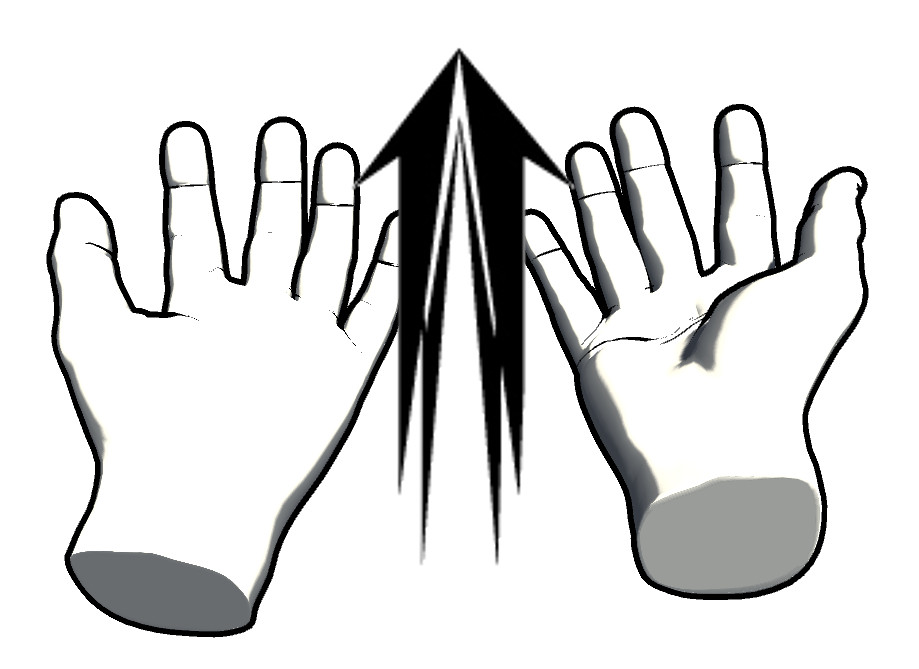
\includegraphics[height=0.08\textheight]{bilder/geste_menu} & Menu \\
		�bersicht & Scrollen & 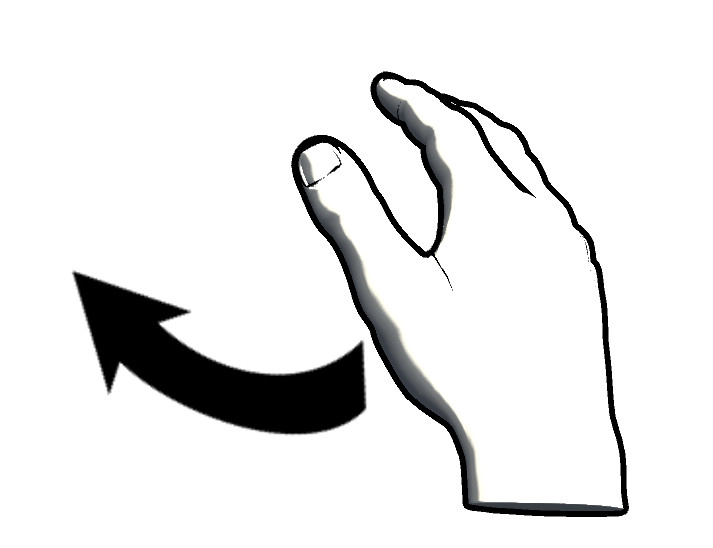
\includegraphics[height=0.08\textheight]{bilder/geste_scroll} & - \\
		Detail & Skalieren des aktiven Bildes & 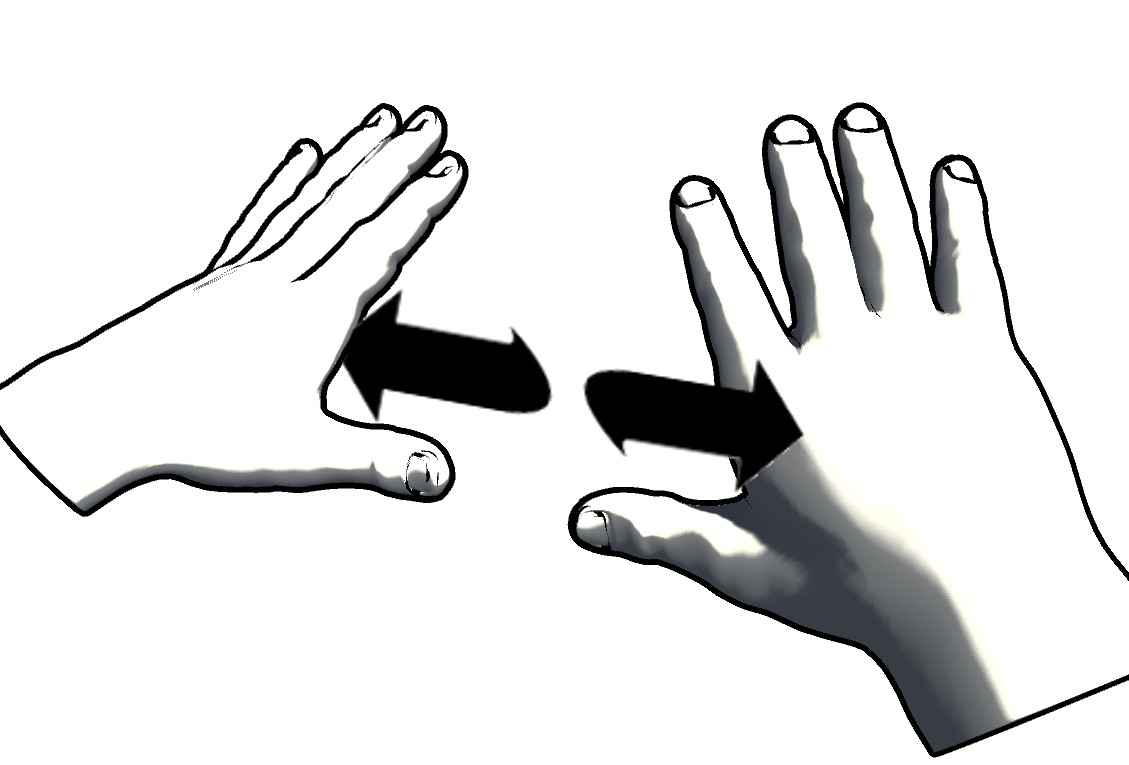
\includegraphics[height=0.08\textheight]{bilder/geste_scale} & - \\
		Detail & Rotieren des aktiven Bildes & 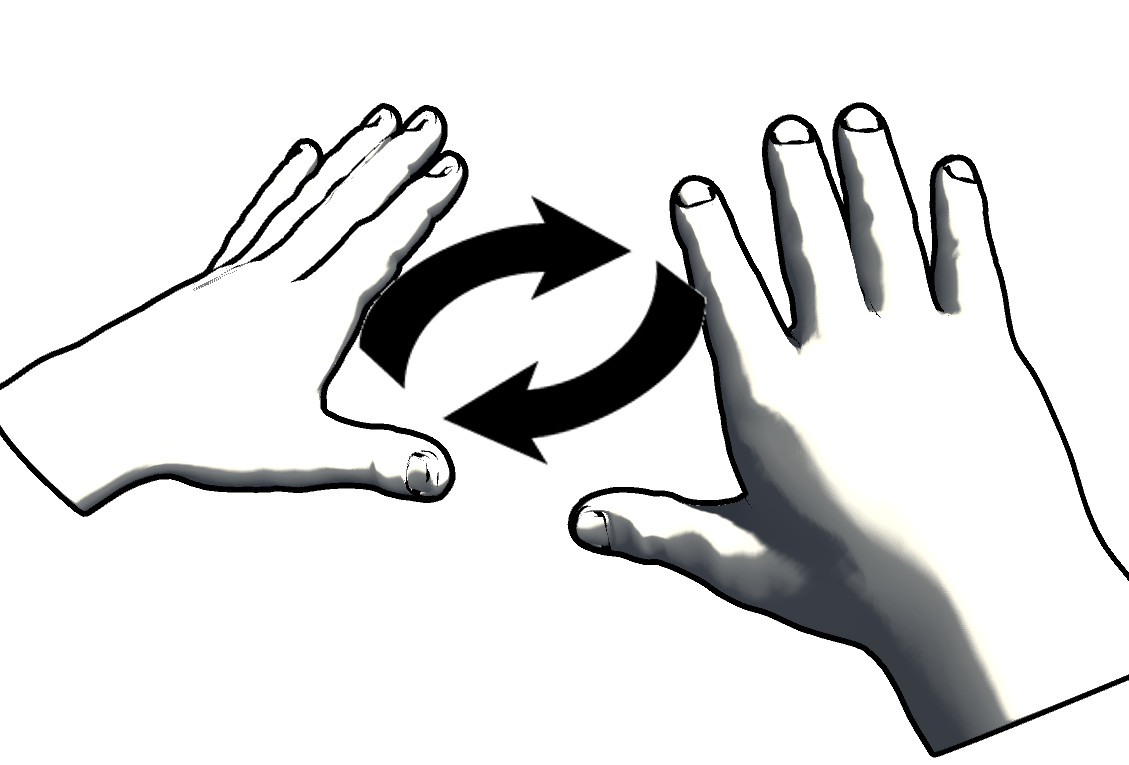
\includegraphics[height=0.08\textheight]{bilder/geste_rotate} & - \\
		�berall & Anzeigen von kontextsensitiven Statistiken & 
\includegraphics[height=0.08\textheight]{bilder/geste_statistics} & - \\
		Dialog & Annehmen / Ablehnen & 
\includegraphics[height=0.08\textheight]{bilder/geste_daumen} & - \\
		Detail & Ansicht verlassen & 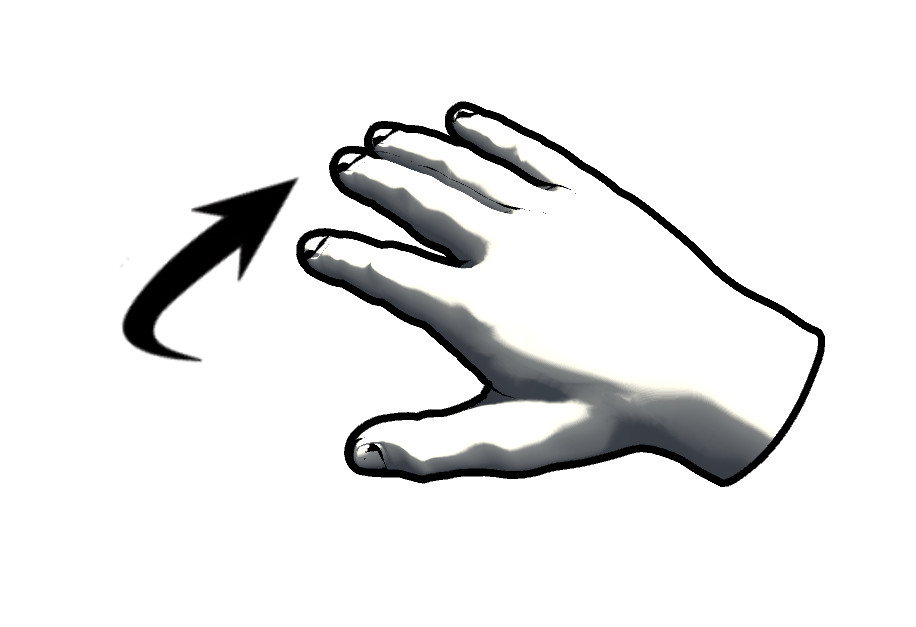
\includegraphics[height=0.08\textheight]{bilder/geste_weg} & - \\
	\end{tabular}
\end{table}

%\chapter{Prototyp}

In der Vorbereitungsphase wurde ein Prototyp geschrieben, um zu testen, ob Unity in der Lage ist, Bilder und Musik so zu manipulieren, wie es die Anforderungen verlangen.

\section{Implementierung}

Der Prototyp besteht aus zwei Teilen: dem Unity-Programm und dem Indexer, der im 
Hintergrund Infos �ber Dateien sammelt. Zwischen den beiden Prozessen gibt es eine 
dateibasierte SQLite Datenbank, auf die mit normalem SQL oder ORM-Modellen zugegriffen 
werden kann.

Um Bilddateien zu analysieren, wird ImageMagick, welches bereits eine Vielzahl von 
Kennwerten zur�ckgibt, verwendet, da dieses �ber ein praktisches C\#-Interface 
verf�gt.

Musikdateien werden noch nicht analysiert. Dies kann jedoch mithilfe des jMIR-Projekts, der VAMP-Plugins und der Echo Nest API erreicht werden. Die Visualisierung der Musik wurde mit der NAudio Library realisiert - es ist allerdings m�glich, die n�tigen Werte direkt �ber die Unity-API zu ermitteln.

Alles in allem zeigt das Unity-Programm, dass es ohne Ruckeln m�glich ist, 100 Bilder zu laden und zu 
sortieren. Die anf�nglichen +100 Draw-Calls konnten auf 2 reduziert werden.

\section{Probleme}

In Sachen Bilder gibt es ein Problem, das es zu �berwinden gilt: Unity erlaubt es nicht, 
Texturen asynchron zu laden. Texturen der Gr�sse 256x256 brauchen nach einer Optimierung 
etwa 1ms zum Laden, was f�r eine Framerate von 60fps noch verkraftbar ist. Gr�ssere 
Texturen (512, 1024) erreichen jedoch schnell eine Ladezeit von 18-50ms, was sich 
langsam aber sicher bemerkbar macht.

Eine M�glichkeit dieses Problem zu l�sen, findet sich in den nativen Plugins: Es ist in Unity 
m�glich, DirectX (oder OpenGL) Code in C++ zu schreiben. Mit dieser Methode k�nnte man evtl. 
die Texturen besser allozieren.

Einfacher w�re es allerdings, alle n�tigen Bilder einfach vorzuladen.
%\chapter{Organisation}

Dieses Kapitel beschreibt kurz die Stakeholder des Projekts sowie den allgemeinen Aufbau.

\section{Projektbeteiligte}

\begin{table}[H]
	\centering
	\begin{tabular}{p{0.2\textwidth} p{0.3\textwidth} p{0.3\textwidth}}
	\textbf{Name} & \textbf{Funktion} & \textbf{E-Mail Adresse} \\ \midrule
	Simon Meer & Student & simon.meer@students.bfh.ch \\
	Prof. Urs K�nzler & Betreuer & urs.kuenzler@bfh.ch \\
	Yves Petitpierre & Experte & ? \\
	\end{tabular}
\end{table}

\section{Projektmanagement}

Meetings zwischen dem Studenten und dem Betreuer finden jeden zweiten Mittwoch in Biel statt.

Das Projekt wird innerhalb eines Git-Projektes gef�hrt und im Laufe des Projekts entweder auf GitHub.com oder auf das interne Projektmanagement-Tool migriert.

Gearbeitet wird durch den Studenten Montags bis Donnerstags an einem Arbeitsplatz im CPVR Labor in Biel.

\section{Zeitplan}


%\chapter{Testszenarien}

Dieses Kapitel definiert eine Reihe von Tests, mit denen das Projekt gepr�ft werden kann und soll.

\section{Indexer}

\begin{description}
	\item [T1 (Anforderung 6.1)] Der Benutzer f�gt seine ``Eigenen Bilder'' und seinen Windows-Ordner zur Library hinzu.
	\item [ $\blacktriangleright$] Der Indexer durchl�uft den Ordner fehlerfrei und die Anzahl indexierter Files, die er ausgibt, stimmt. 
	\item [T2 (Anforderung 6.2)] Der Benutzer �ffnet die Applikation.
	\item [ $\blacktriangleright$] Alle hinzugef�gten Bilder werden angezeigt und sind korrekt sortiert.
	\item [T3 (Anforderung 6.3)] Der Benutzer schliesst die Applikation und l�scht den Windows-Ordner von der Library und startet den Indexer.
	\item [ $\blacktriangleright$] Die Applikation zeigt beim n�chsten Start nur noch die Dateien im Ordner ``Eigene Bilder''.
\end{description}

\section{Bilder}

\begin{description}
	\item [$\bullet$] Der Benutzer f�gt seine ``Eigenen Bilder'' zur Library hinzu.
	\item [T1 (Anforderung 2.1)] Der Benutzer �ffnet die Applikation IMVR.
		\item [ $\blacktriangleright$] Ein 3D-Karussell (oder anders 3D-Konstrukt) mit seinen Bildern wird angezeigt.
	\item [T2 (Anforderung 2.2)] Der Benutzer �ffnet das Men� und sortiert nach Helligkeit.
		\item [ $\blacktriangleright$] Die Elemente werden neu sortiert und erscheinen geordnet nach Helligkeit.
	\item [T3 (Anforderung 2.4)] Der Benutzer ber�hrt mit den H�nden eines der Bilder.
		\item [ $\blacktriangleright$] Die �bersicht verblasst und das selektierte Bild wird vergr�ssert.
	\item [T4 (Anforderung 3.1)] Der Benutzer bewegt seine H�nde auseinander entsprechend der Gestentabelle.
		\item [ $\blacktriangleright$] Das Bild vergr�ssert sich entsprechend.
	\item [T5)] Der Benutzer wischt mit der Hand entsprechend der Gestentabelle.
		\item [ $\blacktriangleright$] Die Detailansicht wird verlassen und die �bersicht kommt wieder in den Vordergrund.
\end{description}

\section{Musik}

\begin{description}
	\item [T1 (Anforderung 4.1)] Der Benutzer f�gt seine ``Eigene Musik'' zur Library hinzu und startet den Indexer.
	\item [ $\blacktriangleright$] Alle MP3 Dateien mit korrekten ID3-Tags werden laut Log erkannt.
	\item [T2 (Anforderung 4.2)] Der Benutzer �ffnet die Applikation und wechselt in den Musikmodus.
	\item [ $\blacktriangleright$] Die soeben hinzugef�gte Musik erscheint alphabetisch geordnet.
	\item [T4 (Anforderung 1.5)] Der Benutzer �ffnet das Hauptmen� und beendet die Applikation.
		\item [ $\blacktriangleright$] Die Applikation fragt einmal nach und beendet dann.
\end{description}

%
%---------------------------------------------------------------------------

% Selbst�ndigkeitserkl�rung
%---------------------------------------------------------------------------
\cleardoublepage
\phantomsection 
\addcontentsline{toc}{chapter}{Selbst�ndigkeitserkl�rung}
\chapter*{Selbst�ndigkeitserkl�rung}
\label{chap:selbstaendigkeitserklaerung}

\vspace*{10mm} 

Ich/wir best�tige/n, dass ich/wir die vorliegende Arbeit selbstst�ndig und ohne Benutzung anderer als der im Literaturverzeichnis angegebenen Quellen und Hilfsmittel angefertigt habe/n. S�mtliche Textstellen, die nicht von mir/uns stammen, sind als Zitate gekennzeichnet und mit dem genauen Hinweis auf ihre Herkunft versehen. 

\vspace{15mm}

\begin{tabbing}
xxxxxxxxxxxxxxxxxxxxxxxxx\=xxxxxxxxxxxxxxxxxxxxxxxxxxxxxx\=xxxxxxxxxxxxxxxxxxxxxxxxxxxxxx\kill
Ort, Datum:		\> [Biel/Burgdorf], \versiondate \\ \\ 
Namen Vornamen:	\> [Test Peter] 	\> [M�ster R�s�] \\ \\ \\ \\ 
Unterschriften:	\> ......................................\> ...................................... \\
\end{tabbing}

%---------------------------------------------------------------------------

% Glossary
%---------------------------------------------------------------------------
\cleardoublepage
\phantomsection 
\addcontentsline{toc}{chapter}{Glossar}
\renewcommand{\glossaryname}{Glossar}
\printglossary

%---------------------------------------------------------------------------

% Bibliography
%---------------------------------------------------------------------------
\cleardoublepage
\phantomsection 
%\addcontentsline{toc}{chapter}{Literaturverzeichnis}
%\printbibliography

\bibliographystyle{IEEEtranS}
\bibliography{datenbanken/bibliography}{}
%---------------------------------------------------------------------------

% Listings
%---------------------------------------------------------------------------
\cleardoublepage
\phantomsection 
\addcontentsline{toc}{chapter}{Abbildungsverzeichnis}
\listoffigures
\cleardoublepage
\phantomsection 
\addcontentsline{toc}{chapter}{Tabellenverzeichnis}
\listoftables
%---------------------------------------------------------------------------

% Index
%---------------------------------------------------------------------------
\cleardoublepage
\phantomsection 
\addcontentsline{toc}{chapter}{Stichwortverzeichnis}
\renewcommand{\indexname}{Stichwortverzeichnis}
\printindex
%---------------------------------------------------------------------------

% Attachment:
%---------------------------------------------------------------------------
%\appendix
%\settocdepth{section}
%\chapter{Beliebiger Anhang}
\label{chap:bel_anhang}

Phasellus eget velit massa, sed faucibus nisi. Etiam tincidunt libero viverra lorem bibendum ut rutrum nisi volutpat. Donec non quam vitae lacus egestas suscipit at eu nisi. Maecenas non orci risus, at egestas tellus. Vivamus quis est pretium mauris fermentum consectetur. Cras non dolor vitae nulla molestie facilisis. Aliquam euismod nisl eget risus pretium non suscipit nulla feugiat. Nam in tortor sapien. Nam lectus nibh, laoreet eu ultrices nec, consequat nec sem. Nulla leo turpis, suscipit in vulputate a, dapibus molestie quam. Vestibulum pretium, purus sed suscipit tempus, turpis purus fermentum diam, id cursus enim mi a tortor. Proin imperdiet varius pellentesque. Nam congue, enim sit amet iaculis venenatis, dui neque ornare purus, laoreet porttitor nunc justo vel velit. Suspendisse potenti. Nulla facilisi.

%\chapter{Weiterer Anhang}
\label{chap:anhang_B}

\section{Test 1}
Phasellus eget velit massa, sed faucibus nisi. Etiam tincidunt libero viverra lorem bibendum ut rutrum nisi volutpat. Donec non quam vitae lacus egestas suscipit at eu nisi. Maecenas non orci risus, at egestas tellus. Vivamus quis est pretium mauris fermentum consectetur. Cras non dolor vitae nulla molestie facilisis. Aliquam euismod nisl eget risus pretium non suscipit nulla feugiat. Nam in tortor sapien. 

\subsection{Umfeld}
Nam lectus nibh, laoreet eu ultrices nec, consequat nec sem. Nulla leo turpis, suscipit in vulputate a, dapibus molestie quam. Vestibulum pretium, purus sed suscipit tempus, turpis purus fermentum diam, id cursus enim mi a tortor. Proin imperdiet varius pellentesque. Nam congue, enim sit amet iaculis venenatis, dui neque ornare purus, laoreet porttitor nunc justo vel velit. Suspendisse potenti. Nulla facilisi.

%\chapter{Inhalt der CD-ROM}
\label{chap:Inhalt_CDROM}

Inhaltsverzeichnis der beiliegenden CD-ROM, ev. Verzeichnisbaum, etc.
%---------------------------------------------------------------------------

%---------------------------------------------------------------------------
\end{document}

